\begin{abstract}
When only a few images carry labels, should the labels go into the contrastive pretraining loss, as in
supervised contrastive learning (\supcon), or be kept for after self-supervised pretraining on all images
(\simclr)? In an earlier study we found \supcon on the labeled 10\% of CIFAR-10 to be 9 points worse
than \simclr on all images, and attributed this to lost data diversity. We revisit this negative result with a
controlled design: one loss for all methods, equal numbers of gradient steps, a $2{\times}2$ split of
\emph{labels} and \emph{images}, \nSeeds seeds, paired bootstrap tests, and two evaluation protocols (a probe
trained on all labels, and fine-tuning with only the labels that exist). We find that (i) the original gap was
an artefact of counting epochs: an epoch over a ten times smaller pool is ten times fewer steps; (ii) labels buy
speed and unlabeled images buy accuracy: at equal steps, label-only \supcon is far ahead early
(\supconTenLin\% vs.\ \simclrTenLin\% after 970 steps) but saturates near 84\%, while \simclr keeps improving to
\simclrTwoHundredLin\%; (iii) labels used inside the loss are spent: fine-tuned with the same 5,000 labels, a
\simclr encoder reaches \simclrTwoHundredFt\%, against \supconTwoHundredFt\% for \supcon and
\unionTwoHundredFt\% for \supcon on all images with unlabeled images as their own class, no better than
plain supervised training on the labeled images (\ceTen\%); and (iv) the mechanism is
memorisation limited by coverage: \supcon collapses the classes of its labeled images \supconCdnvRatio times more
tightly than those of unseen images, and a random labeled subset is as spread out as the full data set: what it lacks is
coverage of unseen images. The standard all-label linear probe hides the third finding. We also quantify the colour shortcut
behind the effect of colour jitter and a resolution failure of CIFAR-trained encoders on ImageNet photographs.
The practical rule: pretrain on every image without labels, count steps rather than epochs, and spend your
labels last.
\end{abstract}

\section{Introduction}
\label{sec:intro}

Contrastive pretraining learns an image encoder by pulling together two augmented views of the same image
and pushing apart views of different images \citep{chen2020simclr,he2020moco}. It needs no labels. When
labels are available, supervised contrastive learning (\supcon) \citep{khosla2020supcon} uses them to
define more positives: all images of a class are pulled together. With all labels, \supcon is better than
both \simclr and cross-entropy training \citep{khosla2020supcon}.

Most practical problems do not have all labels. They have a small labeled set and a much larger unlabeled
one, and this raises a plain question: \emph{where should the few labels go?} They can go \emph{inside} the
contrastive loss, either by running \supcon on the labeled subset or by mixing labeled and unlabeled images
in one objective \citep{assran2020suncet,inoue2020semi}. Or they can be kept until \emph{after} a
label-free pretraining stage and then used for fine-tuning, as in SimCLR~v2 \citep{chen2020simclrv2}, or
for semi-supervised training \citep{sohn2020fixmatch}.

Prior work gives parts of the answer (\cref{sec:related}), but a controlled comparison has to deal with two
confounds.

\begin{itemize}[leftmargin=1.4em]
\item \textbf{Compute.} A method that trains on the labeled subset and a method that trains on all images do
very different amounts of work if their budgets are counted in passes over their own data: one ``epoch''
over 5,000 images is a tenth of the gradient steps of one epoch over 50,000. Careful studies equalise
iterations \citep{newell2020useful,liu2022self}, but the budget unit is often left unclear: in a small audit
of published comparisons of this kind we could not recover the budget of one arm in 5 of 16 papers, and one
compared arms at equal epochs over pools of different size (\ref{app:audit}).
\item \textbf{Evaluation.} The standard test of a pretrained encoder is a linear probe trained on
\emph{all} training labels \citep{chen2020simclr}. In the label-scarce setting those labels do not exist.
The probe then measures what the features would be worth to someone with an oracle, not what the
practitioner with 5,000 labels can obtain \citep{oliver2018realistic}.
\end{itemize}

This paper removes both confounds. All contrastive methods are written as one loss
(\cref{sec:setup}), and two properties are varied independently in a $2\times2$ design: whether the loss
uses the labels, and whether the pretraining pool is the labeled subset or all images. Every method
receives the same number of gradient steps, from 970 to 97,000, and every encoder is evaluated both with the
all-label probe, which we call the \emph{oracle-label probe}, and with protocols that respect the label
budget. The main experiments use CIFAR-10 with 10\% of the labels (5,000 images), a ResNet-18 and five
seeds; we repeat them on CIFAR-100, on STL-10 with its 100,000 unlabeled images, on Tiny-ImageNet with 200
classes, and with a ResNet-50.

\paragraph{Contributions}
\begin{enumerate}[leftmargin=1.6em]
\item \textbf{A compute-matched $2\times2$ comparison} that separates the use of labels from the choice of
images. It shows that labels inside the loss mainly buy speed. \supcon on the labeled subset is
\R{d:simclr-supcon:lp50:e10}\pt ahead of \simclr after 970 steps, statistically equivalent to it after 9,700
steps, and \R{long:d:simclr-supcon}\pt behind after \R{long:steps} steps
(\cref{sec:results}).
\item \textbf{Evidence that the oracle-label probe overstates label-using encoders.} At 9,700 steps the
oracle-label probe puts a semi-supervised \supcon that trains on all images (\union)
\R{cmp:simclr-union:lp50:e100:diff}\pt ahead of \simclr; fine-tuning on the 5,000 labels puts it
\R{cmp:simclr-union:ft:e100:diff}\pt behind with the default recipe and \R{cmp:simclr-union:fts:e100:diff}\pt behind
with the recipe a practitioner can select, and level with \simclr when each encoder gets its best recipe,
chosen on the test set (\cref{sec:protocol}). With longer training \simclr leads under every probe and fine-tuning recipe, including
that upper bound. Holding out labels before pretraining makes recipe selection possible for the label-using
encoders but does not close the gap, and semi-supervised fine-tuning shrinks all differences to less than one
point.
\item \textbf{A seen/unseen diagnostic.} Comparing the tightness of classes on the labeled images, on the
other training images and on test images shows where the label information ends up. Encoders that use
labels make the labeled images several times tighter than any other images; for \union, the images it trains
on without labels are no tighter than test images (\cref{sec:analysis}).
\end{enumerate}

\paragraph{What the results mean in practice}
Within contrastive pretraining, and in the setting we tested (balanced data, in-distribution or mildly
out-of-distribution unlabeled images, small ResNets), scarce labels should not be spent in a \supcon-style
loss. Pretraining without labels on all images and using the labels afterwards is better, whether
``afterwards'' means fine-tuning, a short \supcon stage (which helps a frozen encoder with a linear head, not
fine-tuning), or semi-supervised training. The last option is
the strongest overall: FixMatch and MixMatch \citep{sohn2020fixmatch,berthelot2019mixmatch} beat every
pretrain-then-fine-tune pipeline in our comparison, and at equal total compute FixMatch from scratch matches
FixMatch started from a contrastive encoder (\cref{sec:where}). We say so plainly,
because the question of this paper is where labels belong, not which contrastive method wins.

\section{Related work}
\label{sec:related}

\paragraph{Contrastive learning with and without labels}
\simclr \citep{chen2020simclr} contrasts two views of an image against the other images of a large batch;
MoCo replaces the large batch by a queue of past embeddings \citep{he2020moco,chen2020mocov2}; BYOL and
SimSiam remove the negatives \citep{grill2020byol,chen2021simsiam}. \supcon \citep{khosla2020supcon} treats all
images of a class as positives and, with all labels and a ResNet-50, reports 96.0\% on CIFAR-10 against
93.6\% for \simclr and 95.0\% for cross-entropy. That comparison uses every label; this paper asks what
happens when only a small fraction is available.

\paragraph{Labels inside the loss}
SuNCEt \citep{assran2020suncet} adds a supervised contrastive term on the labeled images to \simclr and
shows that, with 10\% of the ImageNet labels, it matches the semi-supervised accuracy of \simclr with less
than half of the pretraining compute. \citet{inoue2020semi} write supervised and unsupervised contrastive
learning as one generalised loss, and \citet{islam2021broad} study joint \simclr and \supcon objectives with
all labels. PAWS \citep{assran2021paws} and S$^4$L \citep{zhai2019s4l} combine self-supervised and supervised
signals in other ways. A second family starts from pseudo-labeling and adds a contrastive regulariser:
CoMatch \citep{li2021comatch}, SimMatch \citep{zheng2022simmatch}, class-aware contrastive semi-supervised
learning \citep{yang2022classaware} and the clustering-based method of \citet{fini2023semi} all combine labels
and instance-level learning successfully, and USB \citep{wang2022usb} standardises their evaluation. Our
\union arm is the simplest member of the first family; we use it as a controlled probe, not as a
competitor to these methods.

\paragraph{Labels after pretraining}
SimCLR~v2 \citep{chen2020simclrv2} pretrains without labels, fine-tunes on the few labels and then distils
the fine-tuned network on unlabeled data; CPC~v2 \citep{henaff2020data} showed earlier that self-supervised
features allow training with far fewer labels. \citet{zoph2020rethinking} compare pretraining with
self-training across label fractions, and \citet{newell2020useful} measure how the benefit of
self-supervised pretraining shrinks as labels grow. These works establish that the pretrain-then-use-labels
recipe is strong. They do not compare it, at matched compute, with putting the same labels inside the
contrastive loss.

\paragraph{Class collapse and transfer}
At the end of supervised training the features of a class collapse to their mean
\citep{papyan2020neural}; \citet{galanti2022role} measure this with the class-distance normalised variance
(CDNV), and \citet{hui2022limitations} show that collapse on training data need not carry over to test data.
For \supcon, \citet{graf2021dissecting} analyse the collapsed optimum, \citet{chen2022perfectly} show that
class collapse hurts transfer and robustness and counter it with a class-conditional instance term, and
\citet{xue2023which} explain collapse through the simplicity bias of gradient descent.
\citet{kornblith2021better} find that losses with tighter class separation give features that transfer worse,
and \citet{zhao2021what} that the within-class invariance of supervised pretraining discards information
that transfer needs. Our diagnostic applies these ideas to the label-scarce case, where the question is
whether tightness on the \emph{labeled} images reaches the \emph{unlabeled} ones.

\paragraph{Coverage and selection of small sets}
Core-set selection picks points that cover the data \citep{sener2018coreset}. For small budgets, typical
examples beat atypical ones \citep{hacohen2022active}, coverage of the embedding space is the right
selection objective \citep{yehuda2022active}, and data pruning should keep easy examples when data are
scarce \citep{sorscher2022beyond,zheng2023coverage}. We do not propose a selection method; we use pools of
controlled coverage to test whether these findings also explain how a labeled pool limits \supcon.

\paragraph{Budgets and evaluation}
\citet{li2020budgeted} argue for comparing methods at a fixed iteration budget, and
\citet{dehghani2022efficiency} show that a single cost indicator can mislead.
\citet{oliver2018realistic} criticise semi-supervised evaluations that tune on validation sets larger than
the labeled set, and \citet{newell2020useful} note that linear evaluation does not predict fine-tuning
performance. \citet{kumar2022lpft} show that fine-tuning can distort pretrained features and propose to
start from a linear probe. For reference, the solo-learn library reports CIFAR-10 linear accuracies between
88.7\% and 92.9\% for eleven self-supervised methods trained much longer than our reference budget
\citep[Table~1]{dacosta2022sololearn}.

\paragraph{What is new here}
\Cref{tab:novelty} places each of our findings next to the closest earlier evidence. The individual
phenomena have precedents. What was missing is (i) a comparison in which labels and images are varied
separately at equal compute, (ii) a demonstration that the choice between the all-label probe and a
label-budget protocol changes the answer, and (iii) a measurement of tightness on labeled, unlabeled and
unseen images for label-scarce pretraining.

\begin{table}[t]
\centering
\small
\caption{Our findings next to the closest prior evidence.}
\label{tab:novelty}
\begin{adjustbox}{max width=\linewidth}
\begin{tabular}{p{0.24\linewidth} p{0.34\linewidth} p{0.38\linewidth}}
\toprule
finding & closest prior evidence & what this paper adds \\
\midrule
Labels in the contrastive loss speed up pretraining &
SuNCEt reaches the accuracy of \simclr with less than half the compute at 10\% ImageNet labels
\citep{assran2020suncet} &
The speed-up is isolated from the choice of images in a $2\times2$ design at equal steps, and followed to
long budgets, where it turns into a deficit \\
\addlinespace
Labels are best used after label-free pretraining &
SimCLR~v2 \citep{chen2020simclrv2}; pretraining versus self-training \citep{zoph2020rethinking} &
A direct, compute-matched comparison with the same labels inside a \supcon loss, including two-stage and
semi-supervised alternatives \\
\addlinespace
The evaluation protocol can change conclusions &
Unrealistic validation sets in semi-supervised learning \citep{oliver2018realistic}; linear evaluation does
not predict fine-tuning \citep{newell2020useful} &
How much the protocol and the split of the labels change the comparison of the same encoders: default, selectable and oracle fine-tuning recipes, and labels held out for selection at two budgets \\
\addlinespace
Tight classes on training data need not generalise &
Collapse on train but not on test \citep{hui2022limitations}; class collapse in \supcon hurts transfer
\citep{chen2022perfectly,kornblith2021better,xue2023which} &
A three-way split (labeled, unlabeled, test) for label-scarce pretraining, with a cross-entropy control \\
\addlinespace
Coverage matters for small pools &
Low-budget active learning and data pruning
\citep{hacohen2022active,yehuda2022active,sorscher2022beyond} &
An intervention on the labeled pool of \supcon at fixed size; coverage explains part of the effect \\
\bottomrule
\end{tabular}
\end{adjustbox}
\end{table}

\section{Setup}
\label{sec:setup}

\subsection{One loss for all contrastive methods}
A batch holds $B$ images. Each is augmented twice, which gives $2B$ views with $\ell_2$-normalised
projections $z_1,\dots,z_{2B}$. Let $n(i)$ be the image from which view $i$ was made. Every image $n$
carries a \emph{group} $g_n$, and two different views are positives when their images are in the same
group:
\begin{equation}
\label{eq:loss}
\mathcal{L} \;=\; \frac{1}{2B}\sum_{i=1}^{2B} \frac{-1}{|P(i)|}\sum_{p\in P(i)}
\log\frac{\exp(z_i^\top z_p/\tau_i)}{\sum_{a\neq i}\exp(z_i^\top z_a/\tau_i)},
\qquad P(i)=\{\,p\neq i : g_{n(p)} = g_{n(i)}\,\}.
\end{equation}
The temperature $\tau_i\in\{\tau_\ell,\tau_u\}$ depends on the anchor: $\tau_\ell$ if image $n(i)$ is used
with its label and $\tau_u$ otherwise. Three choices of groups give the three methods.
\begin{itemize}[leftmargin=1.4em]
\item \textbf{\simclr} \citep{chen2020simclr}: no label is used and every image is its own group
($g_n=n$). $P(i)$ is the other view of the same image, and \cref{eq:loss} is the NT-Xent loss with
temperature $\tau_u$.
\item \textbf{\supcon} \citep{khosla2020supcon}: every image in the batch is labeled and its group is its
class ($g_n=y_n$). \Cref{eq:loss} is the $\mathcal{L}^{\mathrm{sup}}_{\mathrm{out}}$ loss of
\citet{khosla2020supcon} with temperature $\tau_\ell$.
\item \textbf{\union} (\supcon with unlabeled images): labeled images use their class and unlabeled images
are their own group. An unlabeled image is still contrasted against every other view in the batch, so it
supplies negatives and its own instance-level positive; it never claims a class.
\end{itemize}
We use $\tau_\ell=0.1$ and $\tau_u=0.5$, the standard CIFAR values of \supcon and \simclr
\citep{khosla2020supcon}. Because the temperature depends on the anchor, the loss of \union is not symmetric
in a labeled--unlabeled pair: the pair is weighted with $\tau_\ell$ when the labeled view is the anchor and
with $\tau_u$ when the unlabeled one is. \union is close to SuNCEt \citep{assran2020suncet} and to the
generalised loss of \citet{inoue2020semi}. Its temperatures and the share of labeled images per batch (25\%)
were chosen on a validation split of the training set before any test number was computed
(\cref{app:pilot}). Temperature is thus a second difference between the label-free and the label-using
rows of our design; \cref{sec:plateau} shows that swapping the temperatures does not change the picture.
Our implementation of \cref{eq:loss} agrees with the official \supcon code to $10^{-6}$ (\cref{app:impl}).

\subsection{The \texorpdfstring{$2\times2$}{2x2} design}
With a labeled fraction $f$ (10\% unless stated), the label-scarce setting couples two things: the
\emph{labels} that the loss may use and the \emph{images} in the pretraining pool. \Cref{tab:design} varies
them independently. Comparing the rows gives the effect of the labels at a fixed pool. Comparing the columns
gives the effect of the unlabeled images at a fixed use of labels. The labeled subsets are class-balanced
and nested across fractions for a given seed.

\begin{table}[t]
\centering
\small
\caption{The $2\times2$ design. Each cell is one pretraining method; all four receive the same number of
gradient steps.}
\label{tab:design}
\begin{tabular}{lcc}
\toprule
 & pool = the labeled images only & pool = all images \\
\midrule
labels not used in the loss & \simclrsub & \simclr \\
labels used in the loss & \supcon & \union \\
\bottomrule
\end{tabular}
\end{table}

\subsection{Compute accounting}
\label{sec:compute}
\paragraph{Steps, not epochs}
Every contrastive run performs $T=E\cdot\lfloor N/B\rfloor$ gradient steps with batch size $B=512$, where $N$
is the size of the \emph{full} training set, whatever the size of the method's own pool. On CIFAR
($N=50{,}000$) this is $97E$ steps of 1,024 augmented views. We report $E$ from 10 to 1,000, that is, 970 to
97,000 steps, and always state budgets in steps. A method whose pool has 5,000 images simply cycles through
it ten times as often.

The distinction matters. If each method were instead given ``100 epochs'' over its own pool, \supcon on
5,000 images would run $100\cdot\lfloor 5{,}000/512\rfloor = 900$ steps against 9,700 for \simclr on all
images, and the effect of supervision would be mixed with an eleven-fold difference in compute. In our
experiments this alone moves \supcon by \R{d:steps900}\pt (\R{supcon_lab_f0.1_steps900:lp50} at 900 steps
against \R{supcon_lab_f0.1_e100:lp50} at 9,700). We do not claim that the confusion is widespread: in the
audit of \cref{app:audit}, 7 of 17 applicable papers matched or accounted for the difference, 2 compared
arms at equal epochs over pools of different size, and 5 did not state the budget of one arm in a way a
reader can check. Stating budgets in steps or in images processed removes the ambiguity.

\paragraph{Cost per step}
\Cref{tab:compute} lists, for every method, the number of augmented views, forward passes and backward
passes per step, the number of steps at the reference budget and the wall-clock time on one NVIDIA A40.
The three contrastive methods have identical cost. BYOL adds a forward pass through its target network. The
semi-supervised baselines are given the same number of processed views as a 9,700-step contrastive run
unless stated; their per-step composition differs, so we report it explicitly.

\begin{table}[t]
\centering
\small
\caption{Compute accounting on CIFAR-10 with a ResNet-18. ``Reference budget'' is the budget labeled 9,700
steps in the text. FixMatch processes 64 labeled, 448 weakly and 448 strongly augmented unlabeled views per
step; MixMatch needs an extra forward pass to guess labels. Minutes are wall-clock training time on one
NVIDIA A40 with no other job on the GPU.}
\label{tab:compute}
\begin{adjustbox}{max width=\linewidth}
% generated by scripts/make_assets.py -- do not edit
\begin{tabular}{lcccrcc}
\toprule
 & \multicolumn{3}{c}{per step} & & \multicolumn{2}{c}{reference budget} \\
\cmidrule(lr){2-4}\cmidrule(lr){6-7}
method & augmented views & forward passes & backward passes & steps & forward passes ($10^6$) & minutes \\
\midrule
\simclr, \supcon, \union & 1,024 & 1,024 & 1,024 & 9,700 & 9.9 & 12 \\
BYOL & 1,024 & 2,048 & 1,024 & 9,700 & 19.9 & 22 \\
SimSiam & 1,024 & 1,024 & 1,024 & 9,700 & 9.9 & 15 \\
cross-entropy & 512 & 512 & 512 & 9,700 & 5.0 & 6 \\
FixMatch & 64 + 448 + 448 & 960 & 960 & 10,347 & 9.9 & 24 \\
MixMatch & 64 + 2$\times$64 & 320 & 192 & 51,733 & 16.6 & 37 \\
fine-tuning on the 5k (FT-5k) & 128 & 128 & 128 & 2,344 & 0.3 & 1 \\
\bottomrule
\end{tabular}

\end{adjustbox}
\end{table}

\subsection{Evaluation protocols}
\label{sec:protocols}
The encoder is frozen (except in fine-tuning) and its average-pooled features are used in four ways. We
name the protocols once and use the names throughout.
\begin{itemize}[leftmargin=1.4em]
\item \textbf{\lpall, the oracle-label probe.} A linear classifier trained on the features of all
50,000 training images with all their labels \citep{chen2020simclr}. It is the standard measure of
representation quality, but it uses ten times more labels than the setting provides. We also report a
weighted $k$NN classifier with the same 50,000 labels ($k$NN-50k; \citealp{wu2018instance}).
\item \textbf{\lpfive.} The same linear probe trained only on the 5,000 labeled images, the ones the
label-using methods saw during pretraining.
\item \textbf{\ftfive.} Fine-tuning of the whole network on the 5,000 labeled images. The default recipe
starts from the \lpfive solution \citep{kumar2022lpft} and trains for 60 passes over the labeled images
with learning rate 0.01. \Cref{sec:protocol} replaces it by a recipe selected on a split of the 5,000
labels.
\item \textbf{FixMatch-init.} FixMatch \citep{sohn2020fixmatch} started from the pretrained encoder, using
the 5,000 labels and all images without labels.
\end{itemize}
\lpfive, \ftfive and FixMatch-init respect the label budget, and we refer to them together as
\emph{label-budget protocols}. For other fractions we write LP-all and LP-$f$. On STL-10 only 5,000 training
labels exist, so there is no oracle-label probe and every protocol is a label-budget protocol. We consider
the pair (oracle-label probe, label-budget protocol) to be part of the method of this paper: the first says
what an encoder has learned, the second what a practitioner can extract from it, and \cref{sec:protocol}
shows that the two can disagree about which encoder is better.

The linear probes are $\ell_2$-regularised multinomial logistic regressions on standardised features, fitted
with L-BFGS; the regularisation strength is selected on a stratified 20\% of the labels available to the
probe. No design decision in this paper was taken on test data.

\subsection{Data, models and training}
\paragraph{Datasets}
CIFAR-10 and CIFAR-100 \citep{krizhevsky2009cifar} have 50,000 training and 10,000 test images of 32 px; we
use $f=10\%$ (5,000 labels) unless stated and fractions from 1\% to 100\% in \cref{sec:fractions}. STL-10
\citep{coates2011analysis} has 5,000 labeled training images, 8,000 test images and 100,000 unlabeled images
at 96 px. Its unlabeled set comes from a broader distribution than the ten classes, so it tests the
``all images'' column with data that are not curated to match the labels.

\paragraph{Models and optimisation}
The encoder is a ResNet-18 \citep{he2016resnet} with a $3\times3$ stride-1 first convolution and no max-pooling
for 32-px images; for STL-10 the max-pooling layer is kept. A ResNet-50 is used in \cref{sec:datasets}. The
projection head is linear--batch-norm--ReLU--linear with 128 outputs. We train with SGD (momentum 0.9,
weight decay $10^{-4}$, learning rate 0.25 for batch 512, 5\% linear warm-up, cosine decay), the recipe of the
official \supcon code, in mixed precision with the loss computed in float32. The augmentation is the CIFAR
recipe of \citet{chen2020simclr}: random resized crop (scale 0.2--1), horizontal flip, colour jitter of
strength 0.5 applied with probability 0.8, and random grayscale with probability 0.2. Baselines (BYOL,
SimSiam, cross-entropy, FixMatch, MixMatch) and all remaining hyper-parameters are described in
\cref{app:hparams}.

\subsection{Statistics}
\label{sec:stats}
The main configurations are run with five seeds at 9,700 and 19,400 steps and with three seeds elsewhere;
the seed sets the labeled subset, the initialisation and the augmentation stream. We report the mean and
the standard deviation over seeds. Differences between two configurations are tested with a
\emph{hierarchical bootstrap} \citep{efron1993bootstrap}. One replicate first resamples the seeds with
replacement (jointly for the two configurations when they share seeds, because runs with the same seed share
the labeled subset) and then resamples the test images with replacement, using the same resampled images
for both configurations. We draw 100,000 replicates of the difference in mean accuracy and report its
percentile 95\% interval and a two-sided $p$-value. The \R{stats:ntests} planned comparisons of
\cref{tab:stats} form one family, and their $p$-values are adjusted with the Holm--Bonferroni procedure
\citep{holm1979simple}. A statement that two methods perform the same is backed by an equivalence test: two
one-sided tests \citep{schuirmann1987comparison} on the bootstrap distribution with a margin of $\pm1$ point.
With three to five seeds the between-seed variance is estimated coarsely, so we treat intervals as
approximate and do not interpret differences below about one point. Results from a single seed are marked
as such.

\section{Results I: the compute-matched comparison}
\label{sec:results}

\subsection{CIFAR-10 with 10\% labels}
\label{sec:main}

\Cref{fig:budget} follows the four arms of the design from 970 to 97,000 steps under three protocols, and
\cref{tab:main} gives the numbers at four budgets. We first read the results with the oracle-label probe,
because it is the protocol used in most of the literature, and come back to the others in
\cref{sec:protocol}.

\begin{figure}[t]
\centering
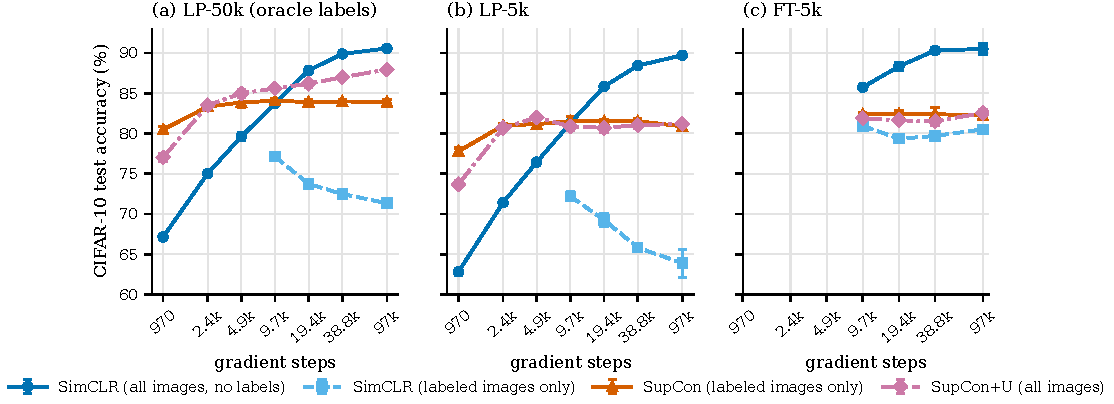
\includegraphics[width=\linewidth]{figures/fig_budget.pdf}
\caption{CIFAR-10, 10\% labels, ResNet-18: test accuracy against the number of gradient steps for the four
arms of the $2\times2$ design. Mean and standard deviation over seeds (five at 9,700 and 19,400 steps,
three elsewhere). (a) With the oracle-label probe, \supcon is far ahead early, level with \simclr at 9,700
steps and behind afterwards. (b, c) With the 5,000 labels only, \simclr is ahead of both label-using methods
from 9,700 steps on. Fine-tuning was run from 9,700 steps on.}
\label{fig:budget}
\end{figure}

\begin{table}[t]
\centering
\small
\caption{CIFAR-10, 10\% labels, ResNet-18. Test accuracy (\%), mean $\pm$ standard deviation over seeds;
best mean per budget and column in bold. \lpall and $k$NN-50k use all 50,000 labels; \lpfive and \ftfive use
only the 5,000 labels of the budget. All budgets are listed in \cref{tab:budgets}; tests are in
\cref{tab:stats}.}
\label{tab:main}
% generated by scripts/make_assets.py -- do not edit
\begin{tabular}{lccccc}
\toprule
 & & \multicolumn{2}{c}{oracle labels (50k)} & \multicolumn{2}{c}{label budget (5k)} \\
\cmidrule(lr){3-4}\cmidrule(lr){5-6}
method & seeds & LP-50k & $k$NN-50k & LP-5k & FT-5k \\
\midrule
\multicolumn{6}{l}{\emph{9,700 steps}} \\
\quad \simclrsub & 5 & 77.1{\scriptsize$\,\pm\,$0.4} & 74.0{\scriptsize$\,\pm\,$0.3} & 72.2{\scriptsize$\,\pm\,$0.5} & 81.0{\scriptsize$\,\pm\,$0.4} \\
\quad \simclr & 5 & 83.7{\scriptsize$\,\pm\,$0.2} & 79.8{\scriptsize$\,\pm\,$0.2} & 81.3{\scriptsize$\,\pm\,$0.2} & \textbf{85.9}{\scriptsize$\,\pm\,$0.4} \\
\quad \supcon & 5 & 84.1{\scriptsize$\,\pm\,$0.3} & 82.2{\scriptsize$\,\pm\,$0.4} & \textbf{81.5}{\scriptsize$\,\pm\,$0.5} & 82.3{\scriptsize$\,\pm\,$0.1} \\
\quad \union & 5 & \textbf{85.6}{\scriptsize$\,\pm\,$0.1} & \textbf{83.2}{\scriptsize$\,\pm\,$0.3} & 80.9{\scriptsize$\,\pm\,$0.5} & 81.9{\scriptsize$\,\pm\,$0.4} \\
\multicolumn{6}{l}{\emph{19,400 steps}} \\
\quad \simclrsub & 5 & 73.7{\scriptsize$\,\pm\,$0.2} & 71.2{\scriptsize$\,\pm\,$0.3} & 69.2{\scriptsize$\,\pm\,$0.9} & -- \\
\quad \simclr & 5 & \textbf{87.8}{\scriptsize$\,\pm\,$0.2} & \textbf{85.7}{\scriptsize$\,\pm\,$0.3} & \textbf{85.8}{\scriptsize$\,\pm\,$0.2} & \textbf{88.6}{\scriptsize$\,\pm\,$0.4} \\
\quad \supcon & 5 & 83.9{\scriptsize$\,\pm\,$0.3} & 82.4{\scriptsize$\,\pm\,$0.1} & 81.5{\scriptsize$\,\pm\,$0.3} & 82.2{\scriptsize$\,\pm\,$0.2} \\
\quad \union & 5 & 86.2{\scriptsize$\,\pm\,$0.4} & 84.3{\scriptsize$\,\pm\,$0.3} & 80.7{\scriptsize$\,\pm\,$0.6} & 81.7{\scriptsize$\,\pm\,$0.3} \\
\bottomrule
\end{tabular}

\end{table}

\paragraph{Labels buy speed}
After 970 steps \supcon reaches \R{supcon_lab_f0.1_e10:lp50:pm}\% and \simclr \R{simclr_all_e10:lp50:pm}\%, a
gap of \R{d:simclr-supcon:lp50:e10}\pt in favour of the method that uses labels. The gap shrinks to
\R{d:simclr-supcon:lp50:e25}\pt at 2,425 steps and \R{d:simclr-supcon:lp50:e50}\pt at 4,850. At 9,700 steps the
two are level: the difference is \R{cmp:simclr-supcon:lp50:e100:sdiff}\pt (95\% interval
\R{cmp:simclr-supcon:lp50:e100:ci}), and the equivalence test accepts a margin of $\pm1$ point
($p=\R{cmp:simclr-supcon:lp50:e100:tost}$). This agrees with SuNCEt \citep{assran2020suncet}: labels in the
loss reach a given accuracy with much less compute.

\paragraph{The lead does not last}
\supcon stops improving early, because once its 5,000 images are separated by class the loss has little
left to learn from them (\cref{sec:geometry}). It is at \R{supcon_lab_f0.1_e25:lp50}\% after 2,425 steps, \R{supcon_lab_f0.1_e200:lp50}\% after 19,400 and
\R{supcon_lab_f0.1_e400:lp50}\% after 38,800. \simclr keeps climbing: \R{simclr_all_e100:lp50}\% at 9,700 steps,
\R{simclr_all_e200:lp50}\% at 19,400 and \R{simclr_all_e400:lp50}\% at 38,800. It is ahead by
\R{cmp:simclr-supcon:lp50:e200:diff}\pt at 19,400 steps (\R{cmp:simclr-supcon:lp50:e200:ci},
$p\,\R{cmp:simclr-supcon:lp50:e200:p}$ after correction) and by \R{cmp:simclr-supcon:lp50:e400:diff}\pt at
38,800 (\R{cmp:simclr-supcon:lp50:e400:ci}). The crossover is therefore not an artefact of a short budget: it
widens as training gets longer. At 97,000 steps \supcon is still at \R{supcon_lab_f0.1_e1000:lp50}\% and
\simclr reaches \R{simclr_all_e1000:lp50}\%, a lead of \R{cmp:simclr-supcon:lp50:e1000:diff}\pt
(\R{cmp:simclr-supcon:lp50:e1000:ci}); after fine-tuning on the 5,000 labels the lead is
\R{cmp:simclr-supcon:ft:e1000:diff}\pt (\R{simclr_all_e1000:ft}\% against \R{supcon_lab_f0.1_e1000:ft}\%,
\R{cmp:simclr-supcon:ft:e1000:ci}). \union, which also sees all images, keeps improving too (\R{union_f0.1_e400:lp50}\% at 38,800
steps and \R{union_f0.1_e1000:lp50}\% at 97,000), because three quarters of each of its batches are unlabeled
images trained by instance discrimination; it stays \R{d:simclr-union:lp50:e1000}\pt behind \simclr.

\paragraph{Reading the $2\times2$}
The two columns of the design answer what the unlabeled images are worth. Without labels the answer is
``a lot, and more with time'': \simclr on all images beats \simclr on the labeled subset by
\R{cmp:simclr-sub:lp50:e100:diff}\pt at 9,700 steps and by \R{cmp:simclr-sub:lp50:e200:diff}\pt at 19,400,
because \simclrsub gets \emph{worse} with more steps (\R{simclr_sub_f0.1_e100:lp50}\% $\to$
\R{simclr_sub_f0.1_e200:lp50}\% $\to$ \R{simclr_sub_f0.1_e1000:lp50}\% at 97,000 steps). With 5,000 images, each one returns in every tenth batch, and instance
discrimination can then be solved with features that identify individual images rather than features shared
within a class: more steps lower the loss on the pool without improving the representation. With labels the unlabeled
images help less: \union beats \supcon by \R{cmp:union-supcon:lp50:e100:diff}\pt and
\R{cmp:union-supcon:lp50:e200:diff}\pt.

The two rows answer what the labels are worth. On the small pool they are worth a great deal: \supcon beats
\simclrsub by \R{cmp:supcon-sub:lp50:e100:diff}\pt at 9,700 steps. On the full pool the answer depends on the
budget: \union is \R{d:simclr-union:lp50:e100}\pt ahead of \simclr at 9,700 steps and
\R{d:simclr-union:lp50:e200}\pt behind at 19,400. So under the oracle-label probe, adding labels to a
contrastive loss that already sees all images helps for short budgets only, and adding unlabeled images to
\supcon always helps a little. \Cref{sec:protocol} shows that the second statement does not survive a change
of protocol.

\subsection{Is the plateau of \supcon a tuning failure?}
\label{sec:plateau}
A plateau after a few thousand steps on 5,000 images could simply mean that \supcon is under-regularised:
9,700 steps are almost a thousand passes over the labeled images. We tested four explanations.

\emph{Temperature.} The rows of the design differ in temperature. Swapping them does not help either
method: \simclr with $\tau=0.1$ reaches \R{simclr_all_t0.1_e100:lp50}\% (default
\R{simclr_all_e100:lp50}\%) and \supcon with $\tau=0.5$ reaches \R{supcon_lab_f0.1_t0.5_e100:lp50}\% (default
\R{supcon_lab_f0.1_e100:lp50}\%) at 9,700 steps (one seed each). A low temperature makes \simclr
concentrate on its most similar negatives, which are often images of the same class, and push them apart;
a high temperature weakens the class-level attraction that \supcon gets from its labels.

\emph{Weight decay and augmentation.} \pending{At 38,800 steps we raised the weight decay of \supcon from
$10^{-4}$ to $5\times10^{-4}$ and $10^{-3}$, strengthened the augmentation (crop scale 0.08--1 and
full-strength colour jitter), and combined both (\cref{tab:reg}). The best variant reaches
\R{reg:best}\%, against \R{supcon_lab_f0.1_e400:lp50}\% for the default.}

\emph{Early stopping.} The best checkpoint along the longest \supcon run, selected with all 50,000 labels and
therefore an upper bound on any early-stopping rule, reaches \R{bestknn:supcon}\% $k$NN accuracy, against
\R{bestknn:simclr}\% for \simclr.

\emph{Learning-rate schedule.} Every budget is a separate run with its own warm-up and cosine schedule, so
no point of \cref{fig:budget} is a truncated longer run.

None of these changes the conclusion that, with 5,000 labeled images, \supcon saturates several points below
where label-free pretraining on all images arrives.

\subsection{Label fraction and budget together}
\label{sec:fractions}
\Cref{fig:wins} extends the comparison to label fractions from 1\% to 100\% and to three budgets. Each cell
is the accuracy of the label-using method minus that of \simclr at the same number of steps, under the
all-label probe (LP-all) and under a probe that sees only the fraction $f$ of the labels (LP-$f$).

\begin{figure}[t]
\centering
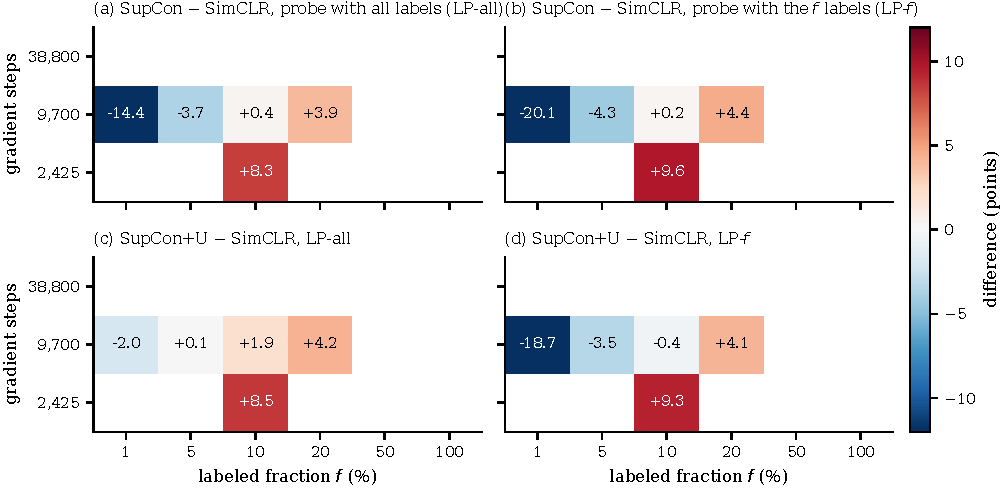
\includegraphics[width=\linewidth]{figures/fig_wins.pdf}
\caption{Which method wins, by label fraction and budget (CIFAR-10, ResNet-18, one seed except $f=10\%$).
Cells show the accuracy of \supcon (a, b) or \union (c, d) minus that of \simclr at the same number of steps;
red means that the label-using method is ahead. LP-all is the oracle-label probe; LP-$f$ uses the same
fraction of labels as pretraining. The numbers behind the chart are in \cref{tab:fraction}.}
\label{fig:wins}
\end{figure}

\pending{Three regions are visible. With few labels and many steps (upper left) \simclr wins under both
probes. With many labels (right) \supcon wins everywhere, in line with the full-label result of
\citet{khosla2020supcon}; the break-even fraction moves to the right as the budget grows. With few steps
(bottom row) the label-using methods win at every fraction, the speed effect of \cref{sec:main}. The LP-$f$
panels are shifted towards \simclr relative to the LP-all panels, most strongly for \union, which is the
protocol effect studied in \cref{sec:protocol}.}

\subsection{Other datasets and a larger encoder}
\label{sec:datasets}

\begin{table}[t]
\centering
\small
\caption{The four arms on CIFAR-100, on STL-10 and with a ResNet-50 (test accuracy in \%, mean $\pm$
standard deviation over seeds). LP-all uses all training labels and is not available on STL-10, whose
5,000 labels are the whole labeled set; LP-budget and FT-budget use the labels of the budget only.}
\label{tab:datasets}
\begin{adjustbox}{max width=\linewidth}
% generated by scripts/make_assets.py -- do not edit
\begin{tabular}{lrcccc}
\toprule
method & steps & seeds & LP-all & LP-budget & FT-budget \\
\midrule
\multicolumn{6}{l}{\emph{CIFAR-100, 10\% labels (5,000), ResNet-18}} \\
\quad \simclrsub & 9,700 & 3 & 44.5{\scriptsize$\,\pm\,$0.2} & 33.0{\scriptsize$\,\pm\,$0.1} & 42.6{\scriptsize$\,\pm\,$0.3} \\
\quad \simclr & 9,700 & 3 & 54.6{\scriptsize$\,\pm\,$0.4} & 43.5{\scriptsize$\,\pm\,$0.3} & \textbf{50.7}{\scriptsize$\,\pm\,$1.3} \\
\quad \supcon & 9,700 & 3 & 51.0{\scriptsize$\,\pm\,$0.7} & 41.8{\scriptsize$\,\pm\,$0.8} & 44.4{\scriptsize$\,\pm\,$0.6} \\
\quad \union & 9,700 & 3 & \textbf{56.1}{\scriptsize$\,\pm\,$0.7} & \textbf{44.9}{\scriptsize$\,\pm\,$0.2} & 47.7{\scriptsize$\,\pm\,$1.1} \\
\quad \simclr & 19,400 & 3 & \textbf{59.5}{\scriptsize$\,\pm\,$0.2} & \textbf{51.0}{\scriptsize$\,\pm\,$0.4} & \textbf{55.1}{\scriptsize$\,\pm\,$0.8} \\
\quad \supcon & 19,400 & 3 & 50.2{\scriptsize$\,\pm\,$0.2} & 40.3{\scriptsize$\,\pm\,$0.5} & 43.0{\scriptsize$\,\pm\,$0.7} \\
\quad \union & 19,400 & 3 & 57.5{\scriptsize$\,\pm\,$0.5} & 41.3{\scriptsize$\,\pm\,$0.5} & 43.7{\scriptsize$\,\pm\,$0.7} \\
\addlinespace
\multicolumn{6}{l}{\emph{STL-10, 5,000 labels + 100,000 unlabeled images, 96 px, ResNet-18}} \\
\quad \simclrsub & 20,500 & 3 & -- & 70.9{\scriptsize$\,\pm\,$0.4} & 82.3{\scriptsize$\,\pm\,$0.4} \\
\quad \simclr & 20,500 & 3 & -- & \textbf{84.4}{\scriptsize$\,\pm\,$0.7} & \textbf{89.4}{\scriptsize$\,\pm\,$0.4} \\
\quad \supcon & 20,500 & 3 & -- & 83.8{\scriptsize$\,\pm\,$0.2} & 84.1{\scriptsize$\,\pm\,$0.3} \\
\quad \union & 20,500 & 3 & -- & 83.7{\scriptsize$\,\pm\,$0.4} & 83.5{\scriptsize$\,\pm\,$0.4} \\
\quad \simclrsub & 41,000 & 3 & -- & 69.3{\scriptsize$\,\pm\,$0.4} & 82.6{\scriptsize$\,\pm\,$0.3} \\
\quad \simclr & 41,000 & 3 & -- & \textbf{86.9}{\scriptsize$\,\pm\,$1.1} & \textbf{90.8}{\scriptsize$\,\pm\,$0.2} \\
\quad \supcon & 41,000 & 3 & -- & 83.9{\scriptsize$\,\pm\,$0.6} & 84.5{\scriptsize$\,\pm\,$0.4} \\
\quad \union & 41,000 & 3 & -- & 84.3{\scriptsize$\,\pm\,$0.6} & 84.2{\scriptsize$\,\pm\,$0.4} \\
\addlinespace
\multicolumn{6}{l}{\emph{Tiny-ImageNet, 10\% labels (10,000), 64 px, ResNet-18}} \\
\quad \simclrsub & 19,500 & 3 & 24.4{\scriptsize$\,\pm\,$0.2} & 16.8{\scriptsize$\,\pm\,$0.4} & 26.7{\scriptsize$\,\pm\,$1.3} \\
\quad \simclr & 19,500 & 3 & 37.8{\scriptsize$\,\pm\,$0.4} & 28.5{\scriptsize$\,\pm\,$0.3} & \textbf{35.3}{\scriptsize$\,\pm\,$0.3} \\
\quad \supcon & 19,500 & 3 & 35.6{\scriptsize$\,\pm\,$0.2} & 26.6{\scriptsize$\,\pm\,$0.2} & 28.6{\scriptsize$\,\pm\,$1.0} \\
\quad \union & 19,500 & 3 & \textbf{40.2}{\scriptsize$\,\pm\,$0.2} & \textbf{28.9}{\scriptsize$\,\pm\,$0.3} & 33.6{\scriptsize$\,\pm\,$0.4} \\
\quad \simclrsub & 39,000 & 3 & 21.8{\scriptsize$\,\pm\,$0.1} & 14.2{\scriptsize$\,\pm\,$0.2} & 26.2{\scriptsize$\,\pm\,$0.5} \\
\quad \simclr & 39,000 & 3 & \textbf{42.1}{\scriptsize$\,\pm\,$0.2} & \textbf{33.2}{\scriptsize$\,\pm\,$0.4} & \textbf{37.3}{\scriptsize$\,\pm\,$0.2} \\
\quad \supcon & 39,000 & 3 & 35.3{\scriptsize$\,\pm\,$0.2} & 26.4{\scriptsize$\,\pm\,$0.4} & 28.4{\scriptsize$\,\pm\,$0.1} \\
\quad \union & 39,000 & 3 & 39.5{\scriptsize$\,\pm\,$0.2} & 21.5{\scriptsize$\,\pm\,$1.0} & 30.3{\scriptsize$\,\pm\,$0.9} \\
\addlinespace
\multicolumn{6}{l}{\emph{CIFAR-10, 10\% labels, ResNet-50}} \\
\quad \simclr & 9,700 & 1 & 85.8 & 82.6 & \textbf{85.6} \\
\quad \supcon & 9,700 & 1 & 86.4 & \textbf{82.9} & 83.6 \\
\quad \union & 9,700 & 1 & \textbf{87.2} & 81.2 & 82.4 \\
\quad \simclr & 19,400 & 3 & \textbf{90.0}{\scriptsize$\,\pm\,$0.1} & \textbf{87.8}{\scriptsize$\,\pm\,$0.1} & \textbf{89.4}{\scriptsize$\,\pm\,$0.3} \\
\quad \supcon & 19,400 & 3 & 85.7{\scriptsize$\,\pm\,$0.2} & 82.5{\scriptsize$\,\pm\,$0.2} & 83.2{\scriptsize$\,\pm\,$0.1} \\
\bottomrule
\end{tabular}

\end{adjustbox}
\end{table}

\paragraph{CIFAR-100}
With 10\% labels there are 50 labeled images per class (three seeds). At 9,700 steps \union is the best arm
under the oracle-label probe (\R{c100_union_f0.1_e100:lp50}\%), ahead of \simclr
(\R{c100_simclr_all_e100:lp50}\%) and \supcon (\R{c100_supcon_lab_f0.1_e100:lp50}\%), and it is still first with
\lpfive (\R{c100_union_f0.1_e100:lp5}\% against \R{c100_simclr_all_e100:lp5}\%). After fine-tuning on the 5,000
labels the order is \simclr (\R{c100_simclr_all_e100:ft}\%), \union (\R{c100_union_f0.1_e100:ft}\%), \supcon
(\R{c100_supcon_lab_f0.1_e100:ft}\%). That \lpfive does not yet reverse the order matches CIFAR-10, where at
9,700 steps \simclr and \union are also within a point under \lpfive (\cref{tab:main}): \simclr is still far
from its end point at this budget, and the gap opens only with longer training. \pending{CIFAR-100 at 19,400
steps is in progress.}

\paragraph{STL-10}
STL-10 has no oracle labels, so every protocol uses its 5,000 labels, and its 100,000 unlabeled images are
not restricted to the ten classes. At 20,500 steps, about 100 passes over the 105,000 images and therefore
the counterpart of 9,700 steps on CIFAR, the linear probe does not separate the three arms: \simclr reaches
\R{stl_simclr_all_e100:lp5:pm}\%, \supcon \R{stl_supcon_lab_e100:lp5:pm}\% and \union
\R{stl_union_e100:lp5:pm}\%. The differences, \R{cmp:stl:simclr-supcon:lp50:e100:sdiff}\pt
(\R{cmp:stl:simclr-supcon:lp50:e100:ci}) and \R{cmp:stl:simclr-union:lp50:e100:sdiff}\pt
(\R{cmp:stl:simclr-union:lp50:e100:ci}), are not significant, as on CIFAR-10 at the same number of passes;
the intervals are still too wide to claim equivalence within one point. Fine-tuning
separates them clearly: \simclr reaches \R{stl_simclr_all_e100:ft:pm}\%, \R{cmp:stl:simclr-supcon:ft:e100:diff}\pt
above \supcon (\R{cmp:stl:simclr-supcon:ft:e100:ci}) and \R{cmp:stl:simclr-union:ft:e100:diff}\pt above \union.
$k$NN on the 5,000 labels favours the label-using encoders (\R{stl_supcon_lab_e100:knn}\% against
\R{stl_simclr_all_e100:knn}\% for \simclr), because a nearest-neighbour rule works best when the labeled
images form tight clusters, which is what \supcon makes of them. The seen/unseen gap of
\cref{sec:geometry} appears here too: the CDNV of \supcon is \R{stl_supcon_lab_e100:cdnv_lab} on its labeled
images and \R{stl_supcon_lab_e100:cdnv_test} on test images, against \R{stl_simclr_all_e100:cdnv_lab} and
\R{stl_simclr_all_e100:cdnv_test} for \simclr. The unlabeled images are worth
\R{cmp:stl:simclr-sub:lp50:e100:diff}\pt of \lpfive to \simclr (\simclrsub reaches
\R{stl_simclr_sub_e100:lp5}\%), although many of them show other classes. For reference, cross-entropy on the
5,000 labels reaches \R{stl_ce_e100:clf:pm}\% and FixMatch \R{stl_fixmatch:clf:pm}\%.
At 41,000 steps the crossover of \cref{sec:main} appears on STL-10 as well. \supcon and \union barely move
(\R{stl_supcon_lab_e200:lp5:pm}\% and \R{stl_union_e200:lp5:pm}\% with \lpfive), for the same reason as on
CIFAR-10: their 5,000 labeled images are already separated by class. \simclr climbs to
\R{stl_simclr_all_e200:lp5:pm}\%, \R{cmp:stl:simclr-supcon:lp50:e200:diff}\pt above \supcon
(\R{cmp:stl:simclr-supcon:lp50:e200:ci}) and \R{cmp:stl:simclr-union:lp50:e200:diff}\pt above \union
(\R{cmp:stl:simclr-union:lp50:e200:ci}). After fine-tuning its lead grows to
\R{cmp:stl:simclr-supcon:ft:e200:diff}\pt and \R{cmp:stl:simclr-union:ft:e200:diff}\pt
(\R{stl_simclr_all_e200:ft:pm}\%), and the $k$NN advantage of the label-using encoders is gone
(\R{stl_simclr_all_e200:knn}\% for \simclr against \R{stl_supcon_lab_e200:knn}\% for \supcon).
\pending{(FixMatch from these encoders is in progress.)}

\paragraph{ResNet-50}
With a ResNet-50 the crossover under the oracle-label probe comes later than with a ResNet-18, as expected
from the finding that label-free contrastive learning gains more than supervised training from larger
encoders and longer training \citep{chen2020simclr}. At 9,700
steps \supcon is still slightly ahead (\R{r50_supcon_lab_f0.1_e100:lp50}\% against
\R{r50_simclr_all_e100:lp50}\%, one seed); at 19,400 steps \simclr is clearly ahead
(\R{r50_simclr_all_e200:lp50}\% against \R{r50_supcon_lab_f0.1_e200:lp50}\%; \pending{one seed, two more in
progress}). Under \ftfive
\simclr is ahead already at 9,700 steps (\R{r50_simclr_all_e100:ft}\% against
\R{r50_supcon_lab_f0.1_e100:ft}\%). The larger encoder also makes very short budgets fragile: at 900 steps
\supcon reaches \R{r50_supcon_lab_f0.1_steps900:lp50}\% with learning rate 0.25 but only
\R{r50_supcon_lab_f0.1_steps900_lr0.05:lp50}\% with 0.05 (\cref{tab:r50}): with so few steps and a cosine
schedule, the smaller learning rate leaves the larger network far from convergence.

\section{Analysis}
\label{sec:analysis}

\subsection{Tight classes on labeled images do not reach the others}
\label{sec:geometry}

\paragraph{The diagnostic}
For a set of images $S$ with class labels, let $\mu_c$ be the mean encoder feature of class $c$ in $S$ and
$\sigma_c^2$ the mean squared distance of the features of class $c$ to $\mu_c$. The class-distance
normalised variance \citep{galanti2022role} of $S$ is
\begin{equation}
\label{eq:cdnv}
\mathrm{CDNV}(S) \;=\; \frac{1}{C(C-1)}\sum_{c\neq c'} \frac{\sigma_c^2+\sigma_{c'}^2}{2\,\lVert\mu_c-\mu_{c'}\rVert^2},
\end{equation}
the average over all ordered pairs of the $C$ classes; we compute it on the 512-dimensional encoder
features without normalisation. A small value means tight, well separated classes. We evaluate
\cref{eq:cdnv} on three disjoint sets, each with its own class means: the 5,000 \emph{labeled} training
images, the \emph{other} 45,000 training images, and the 10,000 \emph{test} images. The same three sets are
used for every method, so the numbers are comparable across methods. What differs is the role of the middle
set: \supcon, \simclrsub and cross-entropy on the 5,000 labels never see the other 45,000 images, while
\simclr and \union train on them without labels. The ground-truth labels of the 45,000 images are used only
for this measurement.

\begin{table}[t]
\centering
\small
\caption{Class tightness (CDNV, \cref{eq:cdnv}) on three sets of images, and accuracy of the \lpfive probe on
its own training images and on test images (CIFAR-10, 10\% labels, ResNet-18, 19,400 steps; mean $\pm$
standard deviation over seeds).}
\label{tab:geometry}
\begin{adjustbox}{max width=\linewidth}
% generated by scripts/make_assets.py -- do not edit
\begin{tabular}{lcccccc}
\toprule
 & \multicolumn{3}{c}{CDNV ($\downarrow$ tighter classes)} & & \multicolumn{2}{c}{LP-5k accuracy} \\
\cmidrule(lr){2-4}\cmidrule(lr){6-7}
encoder (19,400 steps) & labeled 5k & other 45k & test 10k & test / labeled & on its 5k & test \\
\midrule
\simclr & 1.58{\scriptsize$\,\pm\,$0.02} & 1.57{\scriptsize$\,\pm\,$0.01} & 1.61{\scriptsize$\,\pm\,$0.01} & 1.0 & 90.7{\scriptsize$\,\pm\,$2.3} & 85.8{\scriptsize$\,\pm\,$0.2} \\
\simclrsub & 6.12 & 5.80 & 5.64 & 0.9 & 80.9 & 69.2{\scriptsize$\,\pm\,$0.9} \\
\supcon & 0.23{\scriptsize$\,\pm\,$0.01} & -- & 0.68{\scriptsize$\,\pm\,$0.01} & 2.9 & 100.0{\scriptsize$\,\pm\,$0.0} & 81.5{\scriptsize$\,\pm\,$0.3} \\
\union & 0.51{\scriptsize$\,\pm\,$0.01} & -- & 1.64{\scriptsize$\,\pm\,$0.01} & 3.2 & 100.0{\scriptsize$\,\pm\,$0.0} & 80.7{\scriptsize$\,\pm\,$0.6} \\
cross-entropy on 5k & 0.00{\scriptsize$\,\pm\,$0.00} & 0.15{\scriptsize$\,\pm\,$0.01} & 0.16{\scriptsize$\,\pm\,$0.00} & 165.2 & 100.0{\scriptsize$\,\pm\,$0.0} & 83.5{\scriptsize$\,\pm\,$0.5} \\
\simclr{}$\to$\supcon & -- & -- & -- & -- & -- & 87.7{\scriptsize$\,\pm\,$0.3} \\
\bottomrule
\end{tabular}

\end{adjustbox}
\end{table}

\begin{figure}[t]
\centering
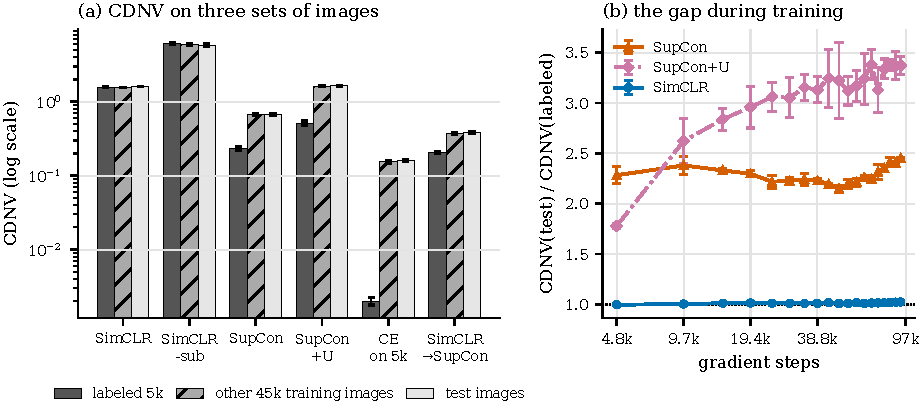
\includegraphics[width=\linewidth]{figures/fig_geometry.pdf}
\caption{(a) CDNV on the labeled images, on the other training images and on test images at 19,400 steps
(log scale, mean $\pm$ standard deviation over seeds). (b) Ratio of the CDNV on test images to the CDNV on
the images the method used with labels (\supcon, \union) or trained on (\simclr), during training.}
\label{fig:geometry}
\end{figure}

\paragraph{What the split shows}
\Cref{tab:geometry} and \cref{fig:geometry}(a) give three observations.

\emph{Label-free pretraining treats all images alike.} For \simclr the CDNV is the same on labeled images
(\R{simclr_all_e200:cdnv_lab}), other training images (\R{simclr_all_e200:cdnv_rest}) and test images
(\R{simclr_all_e200:cdnv_test}).

\emph{\supcon is tight where it had labels.} Its CDNV is \R{supcon_lab_f0.1_e200:cdnv_lab} on the labeled
images and \R{supcon_lab_f0.1_e200:cdnv_test} on test images, a ratio of
\R{supcon_lab_f0.1_e200:cdnv_ratio}. The other 45,000 training images, which it never saw, behave like test
images (\R{supcon_lab_f0.1_e200:cdnv_rest}).

\emph{In \union the labels do not spread.} \union trains on all 50,000 images, yet its CDNV is
\R{union_f0.1_e200:cdnv_lab} on the labeled 5,000 and \R{union_f0.1_e200:cdnv_rest} on the 45,000 images it
saw without labels, which is as loose as on test images (\R{union_f0.1_e200:cdnv_test}) and as loose as
\simclr. The joint loss makes the labeled images tight and leaves the unlabeled ones where instance
discrimination puts them. This is the direct reason why \union looks good to a probe that brings fresh
labels for the 45,000 images and gains nothing for a probe restricted to the 5,000.

\paragraph{The gap is not specific to \supcon}
Cross-entropy training on the 5,000 labels shows the same pattern in a stronger form: the labeled images
collapse almost completely (CDNV \R{ce_f0.1_e200:cdnv_lab}) while test images stay at
\R{ce_f0.1_e200:cdnv_test}. The gap between seen and unseen images is therefore ordinary supervised
overfitting to a small labeled set, as described for neural collapse by \citet{hui2022limitations}, and not
a property of the contrastive loss. What is specific to the label-scarce contrastive setting is its
consequence: the labels have been used to fit 5,000 images, and reusing them in a probe or in fine-tuning
adds little. Cross-entropy on the 5,000 labels is in fact tighter on test images than \supcon
(\R{ce_f0.1_e200:cdnv_test} against \R{supcon_lab_f0.1_e200:cdnv_test}) and slightly more accurate
(\cref{tab:where}).

\paragraph{Dynamics}
\Cref{fig:geometry}(b) follows the ratio between the CDNV on test images and on the labeled images during
the longest runs for which it was logged (\R{geomcurve:supcon:n} seeds, checkpoints up to
\R{geomcurve:supcon:laststep} steps). For \supcon the ratio is already
\R{geomcurve:supcon:first} at \R{geomcurve:supcon:firststep} steps, when its accuracy has almost stopped
improving, and keeps rising to \R{geomcurve:supcon:last}; for \union it rises from \R{geomcurve:union:first}
to \R{geomcurve:union:last}; for \simclr, measured between all training images and test images, it stays at
\R{geomcurve:simclr:last}. The labeled images keep getting tighter relative to new images while the accuracy
no longer improves. This is consistent with the plateau of \supcon being reached once the labeled images are
fitted; the evidence is correlational and we do not claim more.

\subsection{Does the coverage of the labeled pool explain the limit of \supcon?}
\label{sec:coverage}
A natural hypothesis is that \supcon on a small pool is limited by how well the pool \emph{covers} the data:
low-budget active learning and data pruning find that coverage is what matters for small sets
\citep{hacohen2022active,yehuda2022active,sorscher2022beyond}. We test it with an intervention that keeps
the pool size at 5,000 images (500 per class) and changes only which images are in it.

\paragraph{Pools and statistics}
Features are taken from a reference encoder and $\ell_2$-normalised. For a pool $S$, the \emph{coverage
radius} is the mean, over test images $x$, of the cosine distance from $x$ to the nearest pool image of the
same class; the \emph{spread} is the mean cosine distance between two pool images of the same class. Both
are averaged over classes (formulas in \cref{app:pools}). We build three families of pools: random; mixtures
in which 25, 50, 75 or 100\% of each class is chosen by greedy $k$-center selection \citep{sener2018coreset},
which favours atypical images, and the rest at random; and mixtures in which 25, 50, 75 or 100\% consists of
groups of 50 near-duplicates in feature space (``redundant''), and the rest at random. Each pool is drawn
for three seeds, and \supcon and \simclr are trained on it for 9,700 steps. To check that the result does
not depend on measuring distances with a \simclr encoder, all statistics are computed in two reference
spaces: a \simclr encoder trained on all images and a supervised encoder trained on all labels.

\begin{figure}[t]
\centering
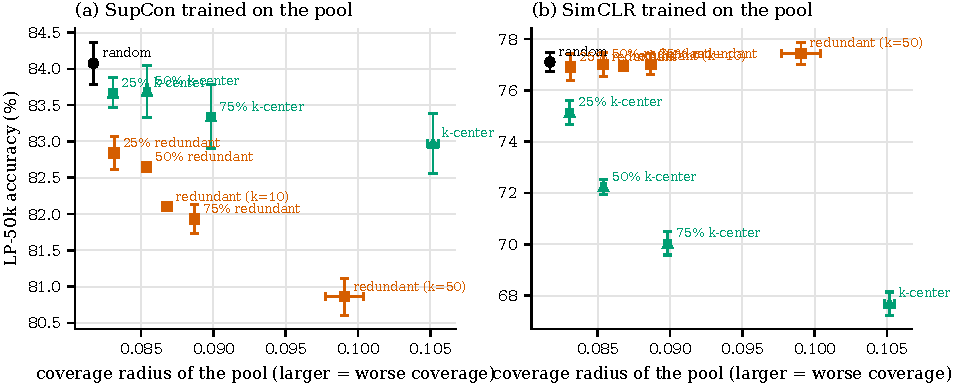
\includegraphics[width=\linewidth]{figures/fig_coverage.pdf}
\caption{Accuracy of (a) \supcon and (b) \simclr trained for 9,700 steps on pools of 5,000 images with
different coverage (CIFAR-10; mean $\pm$ standard deviation over seeds; coverage radius in the \simclr
reference space). Black: random pool; green: mixtures with $k$-center selection; red: mixtures with redundant
groups.}
\label{fig:coverage}
\end{figure}

\paragraph{Result}
\pending{Within the redundant family the picture is clean: as the share of near-duplicates grows, the
coverage radius grows and the accuracy of \supcon falls monotonically, from \R{supcon_lab_f0.1_e100:lp50}\%
for the random pool to \R{supcon_lab_cluster50_f0.1_e100:lp50}\% for the fully redundant one. The
$k$-center family behaves differently: its coverage radius is the largest of all pools, yet \supcon loses
little accuracy (\R{supcon_lab_kcenter_f0.1_e100:lp50}\%), while \simclr trained on the same pool collapses
(\R{simclr_sub_kcenter_f0.1_e100:lp50}\%). Across all pools the rank correlation between coverage radius and
the accuracy of \supcon is \R{rho:all:radius_simclr:supcon} (Spearman, $n=\R{rho:all:radius_simclr:supcon:n}$
pools); within the random and redundant pools it is \R{rho:nokc:radius_simclr:supcon}. The supervised
reference space gives \R{rho:all:radius_supervised:supcon} and \R{rho:nokc:radius_supervised:supcon}. Across
pool sizes from 1\% to 20\%, the partial rank correlation that controls for the pool size is
\R{rho:partial}.} The $k$-center pool is the kind of set that \citet{hacohen2022active} show to be a poor
choice at low budgets for \emph{supervised} learners; here the labels make \supcon robust to it, and the
label-free learner is the one that fails. $k$-center selection picks the images farthest from all others,
that is, atypical images and outliers. Without labels, each of them has few similar images in the pool, so
instance discrimination learns features specific to single images; with labels, the atypical images of a
class are positives of each other, and the class-level positives bridge the gaps between them.

We conclude that coverage explains part of the effect of pool composition, namely the cost of redundancy,
and that no single statistic of the pool predicts the accuracy of both learners. Spread, a natural
candidate, does not separate pools of different size (it is flat from 1\% to 100\% of the data,
\cref{app:pools}) and ranks the $k$-center pool best; it does decrease with redundancy, in line with the
accuracy of \supcon.

\subsection{Labels make colour augmentation less necessary}
\label{sec:jitter}
\simclr is known to depend on colour distortion: without it, two crops of an image can be matched by their
colour histogram alone \citep{chen2020simclr,chen2021intriguing,robinson2021can}. Labels offer another way
out of this shortcut, because two different images of a class do not share a histogram. \Cref{tab:jitter}
removes colour jitter (keeping random grayscale) from the three methods. \simclr loses
\R{jitter:simclr_all_e100}\pt, and \supcon only \R{jitter:supcon_lab_f0.1_e100}\pt. \union loses \R{jitter:union_f0.1_e100}\pt, in between: only the quarter of each batch that is labeled has
class positives, while the unlabeled three quarters are trained by instance discrimination and are exposed to
the colour shortcut like \simclr. Where good augmentations are not
known, for example outside natural images, this is an argument for using labels in the loss that our
accuracy comparison does not capture. The full analysis of colour reliance in \simclr is in
\cref{app:colour}.

\begin{table}[t]
\centering
\small
\caption{Removing colour jitter from the augmentation (CIFAR-10, 10\% labels, 9,700 steps, \lpall accuracy
in \%, mean $\pm$ standard deviation over seeds; the change is computed per seed).}
\label{tab:jitter}
% generated by scripts/make_assets.py -- do not edit
\begin{tabular}{lcccc}
\toprule
method & seeds & full augmentation & without colour jitter & change \\
\midrule
\simclr & 1 & 83.9 & 77.1 & -6.8 \\
\supcon & 1 & 84.0 & 82.7 & -1.3 \\
\bottomrule
\end{tabular}

\end{table}


\section{Limitations}
\label{sec:limits}

We state the limits of each claim rather than a list of further experiments.
\begin{itemize}[leftmargin=*]
\item \textbf{Scale and budget.} All runs use 32-pixel images, mostly a ResNet-18, and at most 19,400 steps. The
crossover of \cref{sec:trap} is a statement about this range of budgets; we do not know how the picture changes
at ImageNet scale, where \citet{cole2022when} observe that more pretraining images stop helping beyond a few
hundred thousand. The epoch trap, being a statement about step counts, does not depend on scale.
\item \textbf{One way to combine labels and images.} We tested one family of semi-supervised contrastive
objectives (\cref{eq:loss}, two batch compositions). Methods that use the labels only late in pretraining, that
weight the supervised term down over time, or that propagate labels to unlabeled images
\citep{assran2021paws,sohn2020fixmatch} may avoid spending the labels; our claim is about putting the labels into
a \supcon-style loss from the start.
\item \textbf{Fine-tuning recipe.} We used one fine-tuning recipe for all encoders. A recipe tuned for
\supcon-pretrained encoders might recover part of the gap; we did not tune it, because the same recipe gains
several points on \simclr encoders.
\item \textbf{Class balance.} CIFAR-10 and CIFAR-100 are balanced and our labeled subsets are stratified. With
imbalanced labels, label-only \supcon would also see a skewed class distribution, and we have not tested
whether coverage or imbalance would then dominate.
\item \textbf{The coverage experiment} uses one seed per pool and a reference encoder that was itself trained
on CIFAR-10, so coverage is measured in a learned space. We show that coverage tracks accuracy across pool
constructions where spread does not; we do not show that it is the only factor.
\item \textbf{Which photometric transform matters.} Our colour analysis separates colour jitter from grayscale,
but not brightness, contrast, saturation and hue from one another.
\item \textbf{Baselines} are budget-matched rather than tuned to convergence. Even so, MixMatch and FixMatch are the most
accurate methods in this study; with its original schedule the margin would be larger. Our results say how to use
labels within contrastive pretraining, not which semi-supervised method is best.
\end{itemize}

\section{Conclusion}
\label{sec:conclusion}

A 9-point deficit of supervised contrastive learning with 10\% labels turned out to be a 21-fold deficit in
training steps. Once compute is matched, a clearer picture appears. Labels inside the contrastive loss make an
encoder learn much faster, but on a small labeled pool it memorises its images and stops improving, while
\simclr on all images keeps getting better. And labels that have been memorised during pretraining cannot be
used a second time: with the 5,000 labels that exist, an encoder pretrained without them and fine-tuned with them
is the best choice. For practitioners this gives three rules: compare methods at equal steps, never drop an
image from the pretraining pool, and spend your labels last.

\bibliography{references}
\bibliographystyle{tmlr}

\setcounter{table}{0}\setcounter{figure}{0}\setcounter{equation}{0}
\renewcommand{\thetable}{A.\arabic{table}}\renewcommand{\thefigure}{A.\arabic{figure}}\renewcommand{\theequation}{A.\arabic{equation}}

\section{Implementation checks}
\label{app:impl}

\paragraph{Augmentation on the GPU}
Every transform draws its random parameters per image, as \texttt{torchvision} does, but processes a whole
batch at once on the GPU. With fixed parameters we compared each operation with
\texttt{torchvision.transforms.functional} on 64 random images: brightness, saturation, hue and grayscale
match exactly; contrast to $6\times10^{-8}$; resized crop (bilinear) and crop with flip to
$1.2\times10^{-7}$. The test is part of the repository.

\paragraph{Loss}
\Cref{eq:loss} was compared with the official \supcon implementation on random embeddings. The maximum
absolute difference is $0$ when all images are labeled (\supcon), $4.8\times10^{-7}$ when none is (NT-Xent),
and $9.5\times10^{-7}$ when half of the batch is labeled (\union, compared with the official code and an
explicit mask).

\needspace{0.45\textheight}
\section{Hyper-parameters}
\label{app:hparams}
\Cref{tab:hparams} lists the hyper-parameters of every method and evaluation protocol.

\begin{table}[!h]
\centering
\small
\caption{Hyper-parameters of all methods (ResNet-18 on CIFAR unless stated). One contrastive step processes
1,024 augmented views.}
\label{tab:hparams}
\begin{adjustbox}{max width=\linewidth}
\begin{tabular}{l l}
\toprule
\simclr, \supcon, \union & SGD, momentum 0.9, lr 0.25 (batch 512), weight decay $10^{-4}$, 5\% warm-up + cosine; 970--97,000 steps \\
 & (9,700 unless stated); $\tau_u=0.5$, $\tau_\ell=0.1$; \union draws 25\% of each batch from the labeled images \\
projection head & Linear(512, 512, no bias)--BN--ReLU--Linear(512, 128); ResNet-50: 2,048 hidden units \\
augmentation & crop (scale 0.2--1), flip, colour jitter (0.4, 0.4, 0.4, 0.1; $p=0.8$), grayscale ($p=0.2$) \\
\simclr{}$\to$\supcon & second stage: \supcon on the labeled images, lr 0.02, 485 steps (2,425 and 9,700 also tested) \\
STL-10 & as above at 96 px; the max-pooling layer after the first convolution is kept; $N=105{,}000$ (205 steps per ``epoch'') \\
Tiny-ImageNet & as above at 64 px with the max-pooling layer; $N=100{,}000$ (195 steps per ``epoch''); 10,000 labels \\
BYOL & SGD, lr 0.24, weight decay $5\times10^{-4}$; projector and predictor 4096--256; target momentum 0.99$\to$1 (cosine) \\
SimSiam & SGD, lr 0.06, weight decay $5\times10^{-4}$; projector 2,048 with BN on the output; predictor 512 at constant lr \\
cross-entropy & SGD with Nesterov momentum, lr 0.2 (batch 512), weight decay $5\times10^{-4}$; crop with padding (size/8) + flip \\
FixMatch & 64 labeled + 448 unlabeled images per step, threshold 0.95, RandAugment + Cutout, SGD-Nesterov lr 0.03, \\
 & weight decay $5\times10^{-4}$, schedule $\cos(7\pi k/16K)$, EMA 0.999; $K=10{,}347$ steps at the reference budget \\
MixMatch & 64 labeled + 64 unlabeled images, two augmentations, $T=0.5$, $\alpha=0.75$, $\lambda_u=75$ (linear ramp), \\
 & Adam lr 0.002, weight decay $0.02\cdot$lr, EMA 0.999; 51,733 steps at the reference budget \\
linear probes & standardised features; multinomial logistic regression, L-BFGS; $\lambda\in\{10^{-6},\dots,10^{-1}\}$ selected \\
 & on 20\% of the labels available to the probe, then refitted on all of them \\
$k$NN & cosine similarity, $k=200$, weights $\exp(s/0.1)$ \\
\ftfive (default) & linear-probe initialisation, SGD-Nesterov lr 0.01, weight decay $5\times10^{-4}$, batch 128, \\
 & 60 passes over the labeled images, crop with padding + flip \\
\ftfive (tuned) & head: LP or random; lr: 0.003, 0.01, 0.03, 0.1; passes: 30, 60, 120; regulariser: none, label smoothing 0.1, \\
 & mixup ($\alpha=0.2$) (72 recipes); widened grid: lr also 0.3 and passes also 240 (120 recipes), used for \supcon \\
 & and \union and for the held-out arm; at 9,700 steps the oracle search of \supcon and \union uses heads LP and random, \\
 & lr 0.03, 0.1, 0.3, passes 60, 120, 240 and label smoothing or mixup (36 recipes); selected on 1,000 of the \\
 & 5,000 labels (or chosen on the test set of seed 0 for the oracle recipe), retrained on all 5,000 \\
self-distillation & teacher: \ftfive (default); student: same architecture, initialised from the pretrained encoder; \\
 & 9,700 steps on all images, batch 512, lr 0.1, weight decay $5\times10^{-4}$, temperature 1 \\
\bottomrule
\end{tabular}
\end{adjustbox}
\end{table}

\section{Choosing the \union variant on a validation split}
\label{app:pilot}
The two design choices of \union (temperatures and the share of labeled images per batch) were made on a
validation split: 5,000 training images were held out, the methods were trained for 4,850 steps on the
remaining 45,000, and the probes were evaluated on the held-out images (\cref{tab:pilot}, one seed). The
test set was not used. Uniform batches, in which about 10\% of the images are labeled, were the second-best
variant, and we kept it as an ablation. On the test set, with three seeds, it reaches \R{unionunif_f0.1_e100:lp50:pm}\%
and \R{unionunif_f0.1_e200:lp50:pm}\% \lpall at 9,700 and 19,400 steps (the chosen variant:
\R{union_f0.1_e100:lp50:pm}\% and \R{union_f0.1_e200:lp50:pm}\%) and \R{unionunif_f0.1_e100:ft:pm}\% and
\R{unionunif_f0.1_e200:ft:pm}\% \ftfive (\R{union_f0.1_e100:ft:pm}\% and \R{union_f0.1_e200:ft:pm}\%). Under the
oracle-label probe the two variants are close (\R{cmp:unionunif-union:lp50:e100:sdiff}\pt at 9,700 steps,
\R{cmp:unionunif-union:lp50:e100:ci}, equivalent within one point; \R{cmp:unionunif-union:lp50:e200:sdiff}\pt at
19,400), but after fine-tuning the uniform variant is better at both budgets
(\R{cmp:unionunif-union:ft:e100:sdiff}\pt, \R{cmp:unionunif-union:ft:e100:ci}, and
\R{cmp:unionunif-union:ft:e200:sdiff}\pt, \R{cmp:unionunif-union:ft:e200:ci}). The validation comparison scored the
variants with linear probes, which hardly separate them, so it could not anticipate this. A likely reason for the
difference is that uniform batches give about 90\% instead of 75\% of every batch to instance discrimination over
all images, the part of the loss that keeps improving the label-free arm. No conclusion changes: after fine-tuning
the uniform variant stays \R{d:simclr-unionunif:ft:e100}\pt (9,700 steps) and \R{d:simclr-unionunif:ft:e200}\pt
(19,400 steps) below \simclr, while under the oracle-label probe at 9,700 steps it is
\R{d:simclr-unionunif:lp50:e100}\pt above it, so with this variant the oracle-label probe would overstate
\union even more.

The same validation split serves to check the length and learning rate of the \simclr{}$\to$\supcon stage of
\cref{sec:where}, which were chosen on test accuracies. A \simclr encoder was
trained on the 45,000 remaining images for 19,400 steps, continued with \supcon on their 10\% labeled subset (4,500
images) for 485, 2,425 or 9,700 steps with three learning rates, and probed on the 5,000 held-out images
(\cref{tab:valstage}). The best setting is 485 steps with learning rate \R{valstage:best:lr}.

\begin{table}[h]
\centering
\small
\caption{Choosing the \simclr{}$\to$\supcon stage on the validation split (45,000 training images, 4,500 labels, one
seed; accuracy in \% on 5,000 held-out training images; the test set is not used). ``LP (4,500 labels)'' is the
counterpart of \lpfive, ``LP (45,000 labels)'' of \lpall.}
\label{tab:valstage}
% generated by scripts/make_assets.py -- do not edit
\begin{tabular}{rccc}
\toprule
second-stage steps & learning rate & LP (4,500 labels) & LP (45,000 labels) \\
\midrule
no second stage & -- & 85.7 & 87.6 \\
485 & 0.005 & 87.2 & 88.7 \\
485 & 0.02 & 87.0 & 88.4 \\
485 & 0.25 & 84.1 & 86.3 \\
2,425 & 0.005 & 86.4 & 87.9 \\
2,425 & 0.02 & 85.5 & 87.5 \\
2,425 & 0.25 & 84.4 & 86.7 \\
9,700 & 0.005 & 84.9 & 86.6 \\
9,700 & 0.02 & 84.7 & 86.4 \\
9,700 & 0.25 & 82.9 & 85.2 \\
\bottomrule
\end{tabular}

\end{table}

\begin{table}[h]
\centering
\small
\caption{Validation-split comparison used to fix the temperatures and the batch composition of \union.}
\label{tab:pilot}
\begin{adjustbox}{max width=\linewidth}
% generated by scripts/make_assets.py -- do not edit
\begin{tabular}{lccc}
\toprule
configuration (validation split, 4,850 steps) & LP (all labels) & $k$NN & LP (10\% labels) \\
\midrule
\simclr, $\tau=0.5$ & 79.2 & 72.8 & -- \\
\simclr, $\tau=0.2$ & 79.8 & 73.8 & -- \\
\simclr, $\tau=0.1$ & 78.9 & 72.4 & -- \\
\supcon, $\tau=0.1$ & 83.0 & 80.9 & 79.7 \\
\supcon, $\tau=0.5$ & 82.4 & 79.6 & 79.3 \\
\union, $\tau=0.1$ for all anchors & 80.9 & 74.4 & 77.4 \\
\union, $\tau=0.5$ for all anchors & 82.5 & 77.7 & 80.2 \\
\union, $\tau_\ell=0.1$, $\tau_u=0.5$, uniform batches & 83.6 & 80.8 & 81.4 \\
\union, $\tau_\ell=0.1$, $\tau_u=0.5$, 50\% labeled per batch & 84.2 & 82.7 & 80.8 \\
\union, $\tau_\ell=0.1$, $\tau_u=0.5$, 25\% labeled per batch (chosen) & 84.5 & 82.8 & 81.6 \\
\bottomrule
\end{tabular}

\end{adjustbox}
\end{table}

\section{Two pitfalls when training \supcon}
\label{app:pitfalls}
Two failure modes cost us several runs and may save time for others.

\paragraph{Half precision overflows at $\tau=0.1$}
With $\tau=0.1$ each exponentiated logit can reach $e^{1/\tau}\approx 22{,}000$, and the denominator of
\cref{eq:loss} sums about a thousand of them. This is far above the largest float16 number (65,504), so a
loss computed under automatic mixed precision returns infinities. We run the forward pass in mixed
precision and compute the loss in float32.

\paragraph{Batch normalisation on the output of the projection head collapses \supcon}
With a batch-normalisation layer after the last linear layer of the head, followed by $\ell_2$
normalisation, all embeddings converged to one point and the loss stayed at $\log(2B-1)$. The official
\supcon head has batch normalisation in the hidden layer only, and we use it for all contrastive methods.

\section{Pool statistics and constructed pools}
\label{app:pools}

\paragraph{Definitions}
Let $\phi(x)$ be the $\ell_2$-normalised feature of image $x$ in the reference space, $S_c$ the pool images
of class $c$ and $T_c$ the test images of class $c$. Then
\begin{align}
\text{coverage radius}(S) &= \frac{1}{C}\sum_{c=1}^{C}\frac{1}{|T_c|}\sum_{x\in T_c}\;\min_{s\in S_c}\bigl(1-\phi(x)^\top\phi(s)\bigr), \\
\text{spread}(S) &= \frac{1}{C}\sum_{c=1}^{C}\frac{1}{|S_c|(|S_c|-1)}\sum_{s\neq s'\in S_c}\bigl(1-\phi(s)^\top\phi(s')\bigr).
\end{align}
The class means of the encoder features in \cref{sec:geometry} are also used for two neural-collapse
statistics that we report in the repository: the deviation from a simplex equiangular tight frame,
$\frac{1}{C(C-1)}\sum_{c\neq c'}\bigl|\cos(\tilde\mu_c,\tilde\mu_{c'})+\tfrac{1}{C-1}\bigr|$ with
$\tilde\mu_c=\mu_c-\frac1C\sum_{k}\mu_k$, and the coefficient of variation of the norms
$\lVert\tilde\mu_c\rVert$ (both are zero for a simplex ETF \citep{papyan2020neural}).

\paragraph{Reference spaces}
The \simclr reference encoder was trained on all images for 9,700 steps (seed 0) and never saw a label. The
supervised reference encoder was trained with cross-entropy on all 50,000 labels.

\paragraph{Constructed pools}
All pools contain exactly 500 images per class.
\emph{Redundant} ($k=10$ or $50$): the images of a class are visited in the random order that defines the
random subset; each visited image that is not yet taken becomes a seed and is added together with its
$k-1$ most similar untaken images of the same class, until 500 images are taken.
\emph{$k$-center}: starting from a random image, greedily add the image whose cosine distance to its nearest
chosen image is largest \citep{sener2018coreset}.
\emph{Mixtures}: a share of 25, 50 or 75\% of each class is chosen by one of the two constructions and the
rest is drawn at random from the remaining images of the class.
Pools are built in the \simclr reference space. \Cref{tab:coverage} lists their statistics and the
accuracies obtained on them.

\begin{table}[h]
\centering
\small
\caption{Pools of 5,000 images with controlled coverage: statistics of the pool and accuracy of \supcon and
\simclr trained on it for 9,700 steps (CIFAR-10; mean $\pm$ standard deviation over seeds).}
\label{tab:coverage}
\begin{adjustbox}{max width=\linewidth}
% generated by scripts/make_assets.py -- do not edit
\begin{tabular}{lccccccc}
\toprule
 & & \multicolumn{2}{c}{coverage radius $\downarrow$} & spread & \multicolumn{2}{c}{\supcon on the pool} & \simclr on the pool \\
\cmidrule(lr){3-4}\cmidrule(lr){6-7}
pool (5,000 images) & seeds & \simclr space & supervised space & & LP-50k & LP-5k & LP-50k \\
\midrule
random & 5 & 0.082 & 0.023 & 0.352 & 84.1{\scriptsize$\,\pm\,$0.3} & 81.5{\scriptsize$\,\pm\,$0.5} & 77.1{\scriptsize$\,\pm\,$0.4} \\
25% k-center & 3 & 0.083 & 0.022 & 0.389 & 83.7{\scriptsize$\,\pm\,$0.2} & 81.1{\scriptsize$\,\pm\,$0.4} & 75.1{\scriptsize$\,\pm\,$0.5} \\
50% k-center & 3 & 0.085 & 0.022 & 0.411 & 83.7{\scriptsize$\,\pm\,$0.4} & 80.1{\scriptsize$\,\pm\,$0.3} & 72.2{\scriptsize$\,\pm\,$0.3} \\
75% k-center & 3 & 0.090 & 0.021 & 0.422 & 83.3{\scriptsize$\,\pm\,$0.4} & 79.2{\scriptsize$\,\pm\,$0.3} & 70.0{\scriptsize$\,\pm\,$0.5} \\
k-center & 2 & 0.105 & 0.021 & 0.426 & 83.2{\scriptsize$\,\pm\,$0.2} & 76.5{\scriptsize$\,\pm\,$0.7} & 67.9{\scriptsize$\,\pm\,$0.4} \\
25% redundant & 3 & 0.083 & 0.023 & 0.340 & 82.8{\scriptsize$\,\pm\,$0.2} & 80.1{\scriptsize$\,\pm\,$0.5} & 76.9{\scriptsize$\,\pm\,$0.5} \\
50% redundant & 2 & 0.085 & 0.024 & 0.332 & 82.6{\scriptsize$\,\pm\,$0.0} & 78.8{\scriptsize$\,\pm\,$0.1} & 76.8{\scriptsize$\,\pm\,$0.5} \\
75% redundant & 2 & 0.089 & 0.024 & 0.324 & 81.8{\scriptsize$\,\pm\,$0.2} & 77.1{\scriptsize$\,\pm\,$0.4} & 76.8{\scriptsize$\,\pm\,$0.1} \\
redundant (k=10) & 1 & 0.087 & 0.025 & 0.335 & 82.1 & 78.3 & 76.9 \\
redundant (k=50) & 2 & 0.099 & 0.024 & 0.317 & 80.8{\scriptsize$\,\pm\,$0.3} & 73.5{\scriptsize$\,\pm\,$0.9} & 77.2{\scriptsize$\,\pm\,$0.1} \\
\bottomrule
\end{tabular}

\end{adjustbox}
\end{table}

\paragraph{Pool size}
For random pools the spread is flat in the pool size while the coverage radius decreases monotonically from
1\% of the data to all of it, in both reference spaces and in pixel space (\cref{tab:poolsize}). Spread therefore
cannot explain why a larger pool is better; the coverage radius can.

\begin{table}[h]
\centering
\small
\caption{Coverage radius and spread of random class-balanced pools of increasing size (CIFAR-10, mean over
seeds; cosine distances in the two reference spaces and in pixel space).}
\label{tab:poolsize}
\begin{adjustbox}{max width=\linewidth}
% generated by scripts/make_assets.py -- do not edit
\begin{tabular}{rrccccccc}
\toprule
 & & & \multicolumn{2}{c}{\simclr space} & \multicolumn{2}{c}{supervised space} & \multicolumn{2}{c}{pixel space} \\
\cmidrule(lr){4-5}\cmidrule(lr){6-7}\cmidrule(lr){8-9}
random pool & images & seeds & radius & spread & radius & spread & radius & spread \\
\midrule
1\% & 500 & 5 & 0.125 & 0.352 & 0.033 & 0.025 & 0.443 & 0.919 \\
5\% & 2,500 & 5 & 0.092 & 0.352 & 0.025 & 0.026 & 0.378 & 0.921 \\
10\% & 5,000 & 5 & 0.082 & 0.352 & 0.023 & 0.025 & 0.356 & 0.920 \\
20\% & 10,000 & 5 & 0.073 & 0.352 & 0.021 & 0.025 & 0.337 & 0.920 \\
50\% & 25,000 & 5 & 0.063 & 0.352 & 0.018 & 0.025 & 0.313 & 0.921 \\
100\% & 50,000 & 1 & 0.057 & 0.351 & 0.016 & 0.025 & 0.296 & 0.920 \\
\bottomrule
\end{tabular}

\end{adjustbox}
\end{table}

\section{Additional results}
\label{app:extra}

\begin{table}[h]
\centering
\small
\caption{All budgets of \cref{fig:budget} (CIFAR-10, 10\% labels, ResNet-18; accuracy in \%, mean $\pm$
standard deviation over seeds).}
\label{tab:budgets}
\begin{adjustbox}{max width=\linewidth}
% generated by scripts/make_assets.py -- do not edit
\begin{tabular}{rcccccccc}
\toprule
 & \multicolumn{2}{c}{\simclr} & \multicolumn{2}{c}{\simclrsub} & \multicolumn{2}{c}{\supcon} & \multicolumn{2}{c}{\union} \\
\cmidrule(lr){2-3}\cmidrule(lr){4-5}\cmidrule(lr){6-7}\cmidrule(lr){8-9}
steps & LP-50k & LP-5k & LP-50k & LP-5k & LP-50k & LP-5k & LP-50k & LP-5k \\
\midrule
970 & 67.1{\scriptsize$\,\pm\,$0.3} & 62.8{\scriptsize$\,\pm\,$0.4} & -- & -- & 80.5{\scriptsize$\,\pm\,$0.4} & 77.8{\scriptsize$\,\pm\,$0.4} & 77.0{\scriptsize$\,\pm\,$0.5} & 73.7{\scriptsize$\,\pm\,$0.4} \\
2,425 & 75.0{\scriptsize$\,\pm\,$0.1} & 71.4{\scriptsize$\,\pm\,$0.2} & -- & -- & 83.3{\scriptsize$\,\pm\,$0.4} & 81.0{\scriptsize$\,\pm\,$0.3} & 83.5{\scriptsize$\,\pm\,$0.4} & 80.7{\scriptsize$\,\pm\,$0.3} \\
4,850 & 79.6{\scriptsize$\,\pm\,$0.5} & 76.4{\scriptsize$\,\pm\,$0.1} & -- & -- & 83.8{\scriptsize$\,\pm\,$0.6} & 81.2{\scriptsize$\,\pm\,$0.4} & 85.0{\scriptsize$\,\pm\,$0.5} & 82.0{\scriptsize$\,\pm\,$0.2} \\
9,700 & 83.7{\scriptsize$\,\pm\,$0.2} & 81.3{\scriptsize$\,\pm\,$0.2} & 77.1{\scriptsize$\,\pm\,$0.4} & 72.2{\scriptsize$\,\pm\,$0.5} & 84.1{\scriptsize$\,\pm\,$0.3} & 81.5{\scriptsize$\,\pm\,$0.5} & 85.6{\scriptsize$\,\pm\,$0.1} & 80.9{\scriptsize$\,\pm\,$0.5} \\
19,400 & 87.8{\scriptsize$\,\pm\,$0.2} & 85.8{\scriptsize$\,\pm\,$0.2} & 73.7{\scriptsize$\,\pm\,$0.2} & 69.2{\scriptsize$\,\pm\,$0.9} & 83.9{\scriptsize$\,\pm\,$0.3} & 81.5{\scriptsize$\,\pm\,$0.3} & 86.2{\scriptsize$\,\pm\,$0.4} & 80.7{\scriptsize$\,\pm\,$0.6} \\
38,800 & 89.9{\scriptsize$\,\pm\,$0.3} & 88.4{\scriptsize$\,\pm\,$0.1} & 72.5{\scriptsize$\,\pm\,$0.1} & 65.8{\scriptsize$\,\pm\,$0.2} & 84.0{\scriptsize$\,\pm\,$0.2} & 81.5{\scriptsize$\,\pm\,$0.4} & 87.0{\scriptsize$\,\pm\,$0.2} & 81.0{\scriptsize$\,\pm\,$0.4} \\
97,000 & 90.5 & 89.6 & -- & -- & 84.0 & 81.2 & -- & -- \\
\bottomrule
\end{tabular}

\end{adjustbox}
\end{table}

{\longtabfont
\setlength{\tabcolsep}{3pt}\setlength{\LTcapwidth}{\linewidth}
\begin{longtable}{@{}lccccc@{}}
\caption{Planned comparisons (CIFAR-10 with 10\% labels unless the group names STL-10; ResNet-18). $\Delta$ is the
difference in mean test accuracy with its hierarchical-bootstrap 95\% interval (100,000 replicates over seeds and
test images); $p$-values are Holm-adjusted over the whole table; the last column is the result of the equivalence
test with a margin of $\pm1$ point. $\Delta$ is computed from unrounded means, so it can differ by 0.1 from the
difference of the rounded means in other tables.}
\label{tab:stats}\\
\toprule
comparison & seeds & $\Delta$ (points) & 95\% CI & $p$ (Holm) & equiv.? \\
\midrule
\endfirsthead
\multicolumn{6}{@{}l}{\emph{\tablename~\thetable{} (continued)}} \\
\toprule
comparison & seeds & $\Delta$ (points) & 95\% CI & $p$ (Holm) & equiv.? \\
\midrule
\endhead
\midrule
\multicolumn{6}{r@{}}{\emph{continued on the next page}} \\
\endfoot
\bottomrule
\endlastfoot
\rawinput generated/tab_stats_rows.tex
\end{longtable}
}

\begin{table}[h]
\centering
\small
\caption{Numbers behind \cref{fig:wins}: accuracy (\%) by label fraction $f$ and budget. \supcon, \union
and fine-tuning use one seed except at $f=10\%$ (three seeds at 2,425 and 38,800 steps, five at 9,700; one for
fine-tuning at 2,425 steps); the \simclr probes use three to five seeds. FT-$f$ was not run with all
labels.}
\label{tab:fraction}
\begin{adjustbox}{max width=\linewidth}
% generated by scripts/make_assets.py -- do not edit
\begin{tabular}{rrccccccccc}
\toprule
 & & \multicolumn{3}{c}{\simclr} & \multicolumn{3}{c}{\supcon} & \multicolumn{3}{c}{\union} \\
\cmidrule(lr){3-5}\cmidrule(lr){6-8}\cmidrule(lr){9-11}
steps & $f$ & LP-all & LP-$f$ & FT-$f$ & LP-all & LP-$f$ & FT-$f$ & LP-all & LP-$f$ & FT-$f$ \\
\midrule
2,425 & 1\% & 75.0 & 64.6 & 64.8 & 69.5 & 55.9 & 55.8 & 76.3 & 62.3 & 59.3 \\
2,425 & 5\% & 75.0 & 68.9 & 74.8 & 80.0 & 75.3 & 76.2 & 80.8 & 76.7 & 77.2 \\
2,425 & 10\% & 75.0 & 71.4 & 79.6 & 83.3 & 81.0 & 82.8 & 83.5 & 80.7 & 81.9 \\
2,425 & 20\% & 75.0 & 72.5 & 84.0 & 86.5 & 85.8 & 86.8 & 84.8 & 83.6 & 85.2 \\
2,425 & 50\% & 75.0 & 74.3 & 89.2 & 89.4 & 88.9 & 90.9 & 84.8 & 84.1 & 89.5 \\
2,425 & 100\% & 75.0 & 75.0 & -- & 89.9 & 89.9 & -- & -- & -- & -- \\
\addlinespace
9,700 & 1\% & 83.7 & 76.2 & 76.6 & 69.3 & 56.2 & 54.5 & 81.7 & 57.5 & 65.4 \\
9,700 & 5\% & 83.7 & 79.9 & 82.4 & 80.0 & 75.7 & 76.7 & 83.8 & 76.5 & 76.4 \\
9,700 & 10\% & 83.7 & 81.3 & 85.7 & 84.1 & 81.5 & 82.4 & 85.6 & 80.9 & 81.9 \\
9,700 & 20\% & 83.7 & 82.1 & 88.7 & 87.6 & 86.5 & 87.9 & 87.9 & 86.2 & 87.2 \\
9,700 & 50\% & 83.7 & 83.2 & 91.9 & 91.4 & 91.2 & 92.7 & 90.9 & 90.4 & 92.1 \\
9,700 & 100\% & 83.7 & 83.7 & -- & 93.5 & 93.5 & -- & -- & -- & -- \\
\addlinespace
38,800 & 1\% & 89.9 & 84.6 & 75.6 & 70.2 & 56.4 & 54.2 & 86.3 & 48.1 & 59.7 \\
38,800 & 5\% & 89.9 & 87.3 & 88.5 & 80.1 & 75.2 & 75.5 & 86.0 & 75.9 & 76.9 \\
38,800 & 10\% & 89.9 & 88.4 & 90.3 & 84.0 & 81.5 & 82.4 & 87.0 & 81.0 & 81.5 \\
38,800 & 20\% & 89.9 & 89.1 & 91.8 & 88.0 & 86.8 & 87.9 & 88.7 & 85.9 & 86.5 \\
38,800 & 50\% & 89.9 & 89.7 & 93.8 & 92.2 & 91.9 & 93.1 & 91.2 & 90.2 & 92.2 \\
38,800 & 100\% & 89.9 & 89.9 & -- & 94.5 & 94.5 & -- & -- & -- & -- \\
\bottomrule
\end{tabular}

\end{adjustbox}
\end{table}

\begin{table}[h]
\centering
\small
\caption{Choosing the fine-tuning recipe (CIFAR-10, 5,000 labels, encoders at 19,400 steps; grid of 72
recipes, widened to 120 recipes, with learning rates up to 0.3 and up to 240 passes, for the oracle choice of
\supcon and \union). ``Label split'': recipe chosen on 1,000 of the 5,000 labels; the selection score is the validation
accuracy. ``Test set (oracle)'': recipe chosen on the test set of seed 0, an upper bound; the selection score
is the test accuracy of seed 0, and the last column reports the other two seeds. ``Recipe of \simclr'': the
label-split choice for \simclr applied to another encoder. Test accuracy is the mean $\pm$ standard deviation
over seeds.}
\label{tab:ftsearch}
\begin{adjustbox}{max width=\linewidth}
% generated by scripts/make_assets.py -- do not edit
\begin{tabular}{lllcc}
\toprule
encoder & recipe chosen on & chosen recipe & range of the selection score over the grid & test accuracy \\
\midrule
\simclr & label split & LP head, lr 0.01, 30 passes, label smoothing & 82.3--89.6 & 89.4{\scriptsize$\,\pm\,$0.1} \\
\simclr & test set (oracle) & LP head, lr 0.01, 120 passes, label smoothing & 85.4--89.8 & -- \\
\addlinespace
\addlinespace
\addlinespace
\supcon & label split & LP head, lr 0.003, 30 passes, none & 93.2--100.0 & 81.3{\scriptsize$\,\pm\,$0.3} \\
\supcon & test set (oracle) & LP head, lr 0.1, 120 passes, mixup & 80.9--87.3 & -- \\
\addlinespace
\union & label split & LP head, lr 0.003, 120 passes, label smoothing & 89.6--100.0 & 82.1{\scriptsize$\,\pm\,$0.1} \\
\addlinespace
\bottomrule
\end{tabular}

\end{adjustbox}
\end{table}

\begin{table}[h]
\centering
\small
\caption{Regularising \supcon at 38,800 steps (CIFAR-10, 10\% labels). The last column is the best $k$NN
accuracy over the checkpoints of the run, an upper bound on early stopping.}
\label{tab:reg}
\begin{adjustbox}{max width=\linewidth}
% generated by scripts/make_assets.py -- do not edit
\begin{tabular}{lccccc}
\toprule
\supcon, 38,800 steps & seeds & LP-50k & LP-5k & $k$NN-50k (final) & $k$NN-50k (best checkpoint) \\
\midrule
default (weight decay $10^{\ensuremath{-}4}$) & 3 & 84.0{\scriptsize$\,\pm\,$0.2} & 81.5{\scriptsize$\,\pm\,$0.4} & 82.4{\scriptsize$\,\pm\,$0.2} & 82.4 \\
weight decay $5\times10^{\ensuremath{-}4}$ & 1 & 84.2 & 81.8 & 82.1 & 82.2 \\
weight decay $10^{\ensuremath{-}3}$ & 1 & 84.4 & 82.2 & 82.8 & 82.9 \\
stronger augmentation & 1 & 83.8 & 81.1 & 82.4 & 82.4 \\
weight decay $5\times10^{\ensuremath{-}4}$ + stronger augmentation & 1 & 83.4 & 80.7 & 81.9 & 81.9 \\
\bottomrule
\end{tabular}

\end{adjustbox}
\end{table}

\begin{table}[h]
\centering
\small
\caption{Steps, architecture and learning rate (CIFAR-10, 10\% labels). 900 steps are ``100 epochs'' over the
5,000 labeled images; 970 steps are ``10 epochs'' over all images.}
\label{tab:r50}
% generated by scripts/make_assets.py -- do not edit
\begin{tabular}{llrcccc}
\toprule
encoder & method & steps & learning rate & seeds & LP-50k & LP-5k \\
\midrule
ResNet-18 & \supcon & 900 & 0.25 & 3 & 79.7{\scriptsize$\,\pm\,$0.8} & 77.2{\scriptsize$\,\pm\,$0.6} \\
ResNet-18 & \supcon & 970 & 0.25 & 3 & 80.5{\scriptsize$\,\pm\,$0.4} & 77.8{\scriptsize$\,\pm\,$0.4} \\
ResNet-18 & \supcon & 9,700 & 0.25 & 5 & 84.1{\scriptsize$\,\pm\,$0.3} & 81.5{\scriptsize$\,\pm\,$0.5} \\
ResNet-18 & \supcon & 19,400 & 0.25 & 5 & 83.9{\scriptsize$\,\pm\,$0.3} & 81.5{\scriptsize$\,\pm\,$0.3} \\
ResNet-18 & \simclr & 970 & 0.25 & 3 & 67.1{\scriptsize$\,\pm\,$0.3} & 62.8{\scriptsize$\,\pm\,$0.4} \\
ResNet-18 & \simclr & 9,700 & 0.25 & 5 & 83.7{\scriptsize$\,\pm\,$0.2} & 81.3{\scriptsize$\,\pm\,$0.2} \\
ResNet-18 & \simclr & 19,400 & 0.25 & 5 & 87.8{\scriptsize$\,\pm\,$0.2} & 85.8{\scriptsize$\,\pm\,$0.2} \\
ResNet-50 & \supcon & 900 & 0.25 & 1 & 73.2 & 68.9 \\
ResNet-50 & \supcon & 900 & 0.05 & 1 & 58.8 & 54.5 \\
ResNet-50 & \supcon & 9,700 & 0.25 & 1 & 86.4 & 82.9 \\
ResNet-50 & \supcon & 19,400 & 0.25 & 2 & 85.7{\scriptsize$\,\pm\,$0.2} & 82.6{\scriptsize$\,\pm\,$0.0} \\
ResNet-50 & \simclr & 970 & 0.25 & 1 & 61.7 & 54.7 \\
ResNet-50 & \simclr & 9,700 & 0.25 & 1 & 85.8 & 82.6 \\
ResNet-50 & \simclr & 19,400 & 0.25 & 2 & 90.0{\scriptsize$\,\pm\,$0.1} & 87.8{\scriptsize$\,\pm\,$0.0} \\
\bottomrule
\end{tabular}

\end{table}

\section{Colour reliance of \simclr}
\label{app:colour}
\Cref{tab:colour} removes the colour augmentations of \simclr one at a time. With crop and flip only, the
encoder reaches \R{simclr_exp2_e100:lp50}\% and loses most of it when the test images are converted to
grayscale (\R{simclr_exp2_e100:linear_acc_gray}\%); its features are closer to the colour histogram of the
image than to the class label (linear CKA \R{simclr_exp2_e100:cka_hist} against
\R{simclr_exp2_e100:cka_label} \citep{kornblith2019cka}). A linear classifier on the $8^3$-bin colour
histogram alone reaches \R{histprobe}\%. Random grayscale removes most of the dependence on colour, and
colour jitter and grayscale together give the default accuracy. These runs use one seed and confirm earlier
reports \citep{chen2020simclr,chen2021intriguing,robinson2021can,geirhos2020shortcut}.

\begin{table}[h]
\centering
\small
\caption{Colour reliance of \simclr under four augmentation pipelines (CIFAR-10, 9,700 steps). ``Gray test''
evaluates the \lpall probe on grayscale test images. CKA is linear centred kernel alignment between the
features and the colour histogram or the one-hot label; histogram $R^2$ is the variance of the histogram
explained by a ridge regression on the features.}
\label{tab:colour}
\begin{adjustbox}{max width=\linewidth}
% generated by scripts/make_assets.py -- do not edit
\begin{tabular}{lcccccc}
\toprule
 & & \multicolumn{2}{c}{LP-50k accuracy} & \multicolumn{3}{c}{colour reliance} \\
\cmidrule(lr){3-4}\cmidrule(lr){5-7}
\simclr augmentation & seeds & colour test & gray test & CKA(histogram) & CKA(label) & histogram $R^2$ \\
\midrule
crop + flip & 1 & 60.9 & 24.5 & 0.57 & 0.16 & 0.64 \\
crop + flip + colour jitter & 1 & 75.9 & 38.2 & 0.47 & 0.28 & 0.48 \\
crop + flip + grayscale & 3 & 77.3{\scriptsize$\,\pm\,$0.4} & 75.8{\scriptsize$\,\pm\,$0.2} & 0.31 & 0.34 & 0.33 \\
crop + flip + colour jitter + grayscale (default) & 5 & 83.7{\scriptsize$\,\pm\,$0.2} & 82.6{\scriptsize$\,\pm\,$0.2} & 0.22 & 0.47 & 0.25 \\
\bottomrule
\end{tabular}

\end{adjustbox}
\end{table}

\section{How published comparisons state their budgets}
\label{app:audit}
To see whether unequal compute is a problem in practice, we read the experimental sections of 26 papers
(2019--2025) in which one arm is trained on a labeled subset, or with a labeled subset, and is compared with
an arm trained on a larger pool. Ten papers turned out not to make such a comparison; among them is
\citet{cole2022when}, whose pools of different size are all used for self-supervised pretraining without
labels. \Cref{tab:audit} classifies the other 16. The reading was done from the text of the papers only,
without their code, by one reader; ``unclear'' means that we could not recover the budget of at least one arm
from the paper, not that the comparison is unfair. The one paper in the category of unmatched comparisons
was read a second time in full (arXiv version 1), which confirmed the verdict: SupCon is trained on the 1\% of
the data that is labeled and SimCLR on 70\%, both for 50 epochs; the paper discusses the difference in the number
of images but not in gradient steps, and it does not state the batch size. The quotations behind every verdict,
with their location, are in the repository.

\begin{table}[h]
\centering
\small
\caption{Budget reporting in 16 published comparisons between a labeled-subset arm and a larger-pool arm.}
\label{tab:audit}
\begin{adjustbox}{max width=\linewidth}
\begin{tabular}{p{0.20\linewidth} p{0.46\linewidth} p{0.30\linewidth}}
\toprule
verdict & papers & typical statement of the budget \\
\midrule
matched or accounted for (7) &
\citet{assran2020suncet}, \citet{assran2021paws}, \citet{zheng2022simmatch}, \citet{fini2023semi},
\citet{newell2020useful}, \citet{liu2022self}, \citet{wang2022usb} &
iterations equalised, cost per iteration equalised, or separate columns for labeled and unlabeled epochs \\
\addlinespace
unequal but disclosed (3) &
\citet{zhai2019s4l}, \citet{Cai2022SemiViT}, \citet{zoph2020rethinking} &
epochs defined on the labeled set, or each arm trained to convergence \\
\addlinespace
equal epochs over pools of different size (1) &
\citet{Benato2023Linking} &
the same number of epochs for every pool, no discussion of steps \\
\addlinespace
unclear (5) &
\citet{chen2020simclrv2}, \citet{henaff2020data}, \citet{li2021comatch}, \citet{berthelot2019mixmatch},
\citet{Zhang2021CoCalibration} &
one ``epochs'' column without a definition, or no budget for the baseline \\
\bottomrule
\end{tabular}
\end{adjustbox}
\end{table}

The trap described in \cref{sec:compute} is therefore not common in this sample: most well-known papers
match iterations or report the two budgets separately. The more frequent issue is that the unit of the
budget is not stated in a way that lets a reader check the match. Our sample is small and leans towards
widely cited self- and semi-supervised papers, so it says little about application papers, where
\citet{Benato2023Linking} is an example of the unmatched comparison.

